% !TeX root = ../thesis.tex

\chapter{随机传值进程模型}\label{ch:rvpc}

由于Uniform Approach是模型无关的概率扩展方法,
我们可以使用该方法概率化扩展其他的进程模型。
本章会对传值进程模型进行概率化扩展。
传值进程模型是经典的进程模型,
在MILNER R的Communication and Concurrency一书\cite{Milner_CCS}中,
也是使用传值的通信并发模型——消息的发送者、接受者和通信媒介——引入并发和通信的概念。
我们选择传值进程模型的一种定义——The Value-Passing Calculus\cite{Fu_VPC}进行扩展。

\section{传值进程模型}
传值进程模型(Value-Passing Calculus)是一种
可以将某个域中的值作为通信的内容,
并且可以在特定逻辑条件执行某个动作的并发进程模型。
一个经典的例子是\cite{Milner_CCS}中的一单元缓冲区,它可以接受、储存、发送消息:
\begin{align*}
   C&\stackrel{def}{=}in(x).C'(x)\\
   C'(x)&\stackrel{def}{=}\overline{out}(x).C
\end{align*}
更普遍的传值进程模型也可以对输入进行逻辑判定,
根据特定的条件执行特定的动作,
通过输入控制进程的执行。我们以进程$A(x)$为例:
$$A(x)=\textrm{if }\varphi(x)\textrm{ then }\overline{a}(f(t))\textrm{ else }B(x)$$
$A(x)$在满足条件$\varphi(x)$时会通过通道$a$输出函数$f(t)$的值,
其中$t$可能是$x$的函数,也可能与$x$无关;若不满足$\varphi(x)$,则执行程序$B(x)$。

传值进程模型赋予了进程传递数据的能力,
我们可以通过进程之间传递的数据来控制进程的执行和进程间的交互,
这种控制能力显著的增强了并发进程模型的表达能力,拓宽了应用场景。
在网络通信中,各种通信协议通过在主机间传值进而控制主机的行为,
通信协议的过程就可以被抽象为传值进程模型,
支持并发的编程语言也可以被解释为传值进程模型,如Erlang\cite{Erlang}。
很多通过传值、计算解决的现实问题也都可以抽象为传值进程模型。


\subsection{The Value-Passing Calculus}\label{ch:vpc}
对传值进程模型的研究很多都会依赖一个\textit{神域},
这个神域是一个领域模型(domain model)或一个逻辑理论(logic theory),
帮组我们进行条件的判定,函数的计算和提供变元的取值范围。
如在执行$A(x)$时,我们会将$\varphi(x)$传给神域,
神域判定是否满足条件,并将判定结果返回给我们,
同样的,我们也会将$f(t)$传给神域,神域帮我们计算这个函数,并将结果返回给我们。
例如,WINSKEL G将变元表达式的取值和计算全部依赖一个集合$V$\cite{Oracle_V},
LIN H依赖一个评估$\rho$完成布尔表达式的判定和表达式的计算\cite{Oracle_rho},
MILNER R对CCS的扩展Value-Passing CCS也没有讨论函数的计算过程和条件的可判定性\cite{Milner_CCS}。
神域通常不包括在传值进程模型中,且通常是未定义的,或只在特定场景下定义。
由于神域的存在,对于这些传值进程模型表达能力的衡量变得十分困难,
FU Y在The Value-Passing Calculus中取缔了神域的概念,
提出了一个封闭的传值进程模型\cite{Fu_VPC}。

The Value-Passing Calculus中的传值进程模型$\mathbb{VPC}_{\mathsf{Th}}$
的语法可以表示为:
\begin{equation}\label{eq:vpc}
   T:=\sum_{i\in I}\varphi_i a(x).T_i|\sum_{i\in I}\varphi_i\overline{a}(t_i).T_i|T|T'|(c)T|\varphi T|!a(x).T|!\overline{a}(t).T
\end{equation}
其中$T$是一个$\mathbb{VPC}_{\mathsf{Th}}$项,$\mathsf{Th}$是可判定的逻辑,
$\varphi_i$是一个布尔表达式,可以通过$\mathsf{Th}$证明或证伪,
若$\mathsf{Th}$可以给出$\varphi_i$的一个证明,记为$\mathsf{Th}\vdash \varphi_i$。
$a(x)$是一个输入前缀,$\overline{a}(t_i)$是一个输出前缀,
我们可以用$\sum_{i\in I}\varphi_i\lambda_i.T_i$来表示$\sum_{i\in I}\varphi_i a(x).T_i$或$\sum_{i\in I}\varphi_i \overline{a}(t).T_i$。
$!a(x).T$和$!\overline{a}(t).T$对应递归操作,$\mu X.E$可以表示为
$(c)(E\{c(z).0/X\}|!\overline{c}(r).E\{c(z).0/X\})$。
其余的表达与第一章CCS语法定义的解释相同。

The Value-Passing Calculus提出了两种迁移语义的描述:具体语义(Concrete Semantics)和符号语义(Symbolic Semantics)。
后文我们只用到了符号语义,因此我们忽略具体语义的相关内容。

$\mathbb{VPC}_{\mathsf{Th}}$的符号迁移语义如图~\ref{fig_vpc}所示。

\begin{figure}[!htbp]
   \small
   \centering
   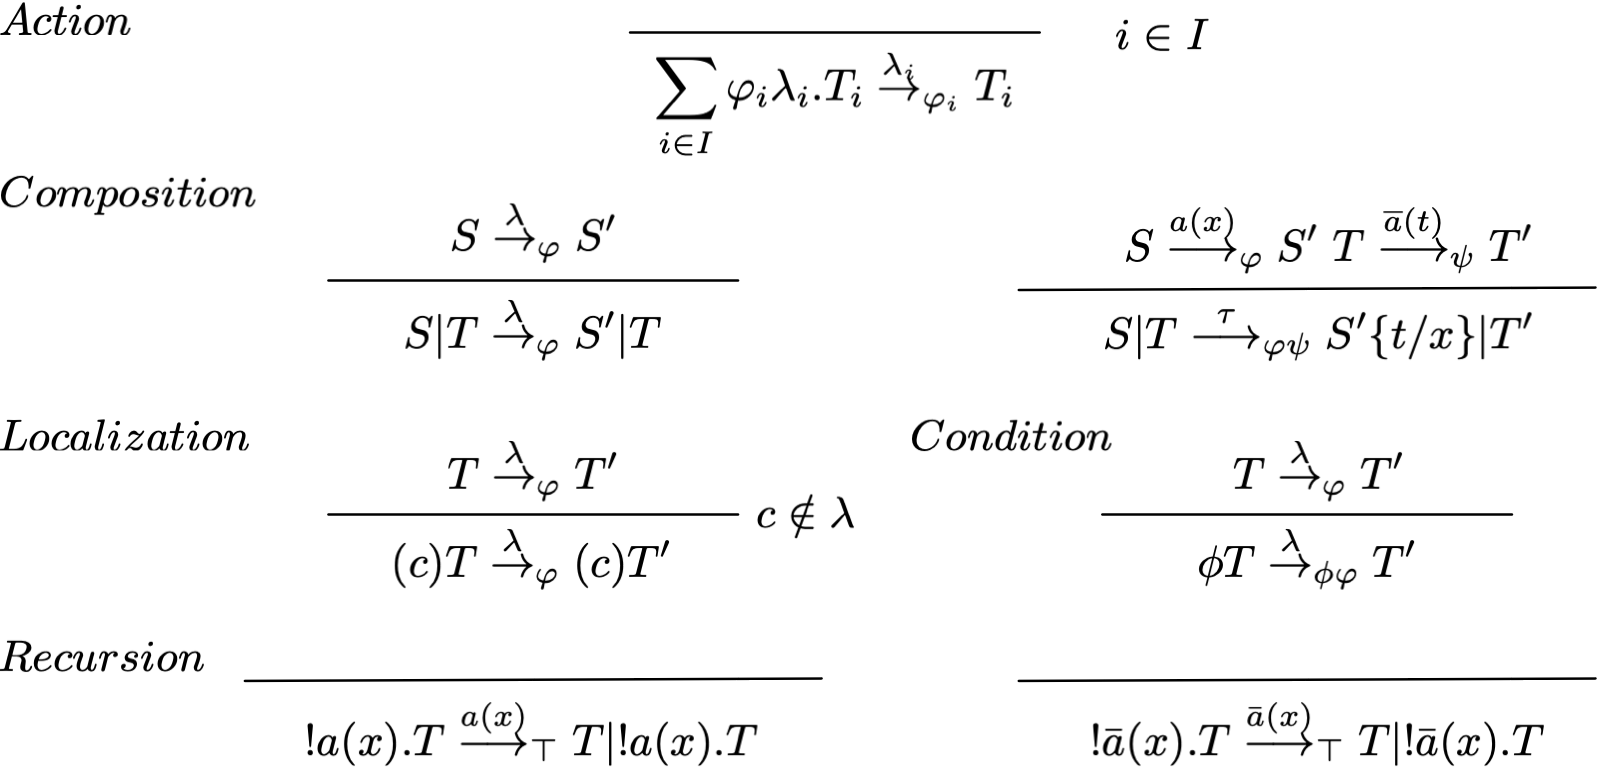
\includegraphics[width=13cm]{../figures/vpc.png}
    \caption[]{$\mathbb{VPC}_{\mathsf{Th}}$的符号迁移语义规则}
    \label{fig_vpc}
\end{figure}
其中,$T=\varphi \lambda.T'$在$\varphi$条件下执行$\lambda$动作到达$T'$状态,
在符号语义下可以写作$T\stackrel{\lambda}{\rightarrow}_{\varphi}T'$。
符号语义中的动作集合$Act=\{a(x),\overline{a}(t)| a\in Chan, x\in \mathsf{V}_{\Sigma}, t\in \mathsf{T}_{\Sigma}\}\cup \{\tau\}$,
$Act$中的元素可以用$\lambda$表示,其中$\mathsf{V}_{\Sigma},\mathsf{T}_{\Sigma}$为可判定逻辑$\mathsf{Th}$中变元的集合和项的集合[引用]。

The Value-Passing Calculus使用可判定的一阶理论判定条件\cite{PA}并
提出了一个图灵完备的数值系统(Numeric System)\cite{Fu_UniformApproach}作为底层模型来实现可计算的函数。
通过这两种方式,将Value-Passing Calculus从神域中解放出来。

\subsection{If Then Else语法符号化}
进程$A(x)$中出现了If Then Else语法,
If Then Else语法实现的分支控制在编程中也是非常重要的组成部分。
在Communication and Concurrency\cite{Milner_CCS}中也多次使用If Then Else语法,
然而在CCS的定义中,我们无法通过CCS代理的语法规则来实现这种分支控制;
书中对分支控制的使用,如第五章(Bisimulation and Observation Equivalence)中对JobShop的建模,
也比较随意,没有严格的定义也没有判断If条件的可判定性。
在FU Y的The Value-Passing Calculus中,
规定了If条件是通过一阶理论$\mathsf{Th}$可判定的布尔表达式,
并说明$\textrm{if }\varphi\textrm{ then }S\textrm{ else }T$
可以被定义为$\varphi S|\urcorner \varphi T$。
以下推论依据The Value-Passing Calculus中对If Then Else语法的定义和$\mathbb{VPC}_{\mathsf{Th}}$的Proof System,
给出If Then Else的变体的符号化定义,在本文的后续章节会统一使用这些符号。

以下推论中$S,T\in \mathcal{T}_{\mathbb{VPC}_\mathsf{Th}}$。
\begin{corollary} 
   $\varphi 0 = 0$
\end{corollary}
\begin{proof}
   $\varphi 0 = \varphi 0 + 0 = \varphi 0 + \top 0 = \varphi 0 + (\varphi \vee \urcorner \varphi)0 = \varphi 0 + \varphi 0 + \urcorner \varphi 0 = \varphi 0 + \urcorner \varphi 0 = (\varphi \vee \urcorner \varphi)0 = \top 0 = 0$
\end{proof}
\begin{corollary}
   $\varphi T = (\varphi T\mid \urcorner \varphi 0)$
\end{corollary}
\begin{proof}
   $\varphi T = (\varphi T\mid 0) = (\varphi T\mid \urcorner \varphi 0)$
\end{proof}
\begin{corollary}
   $S=\urcorner\varphi \varphi T$,则$S=0$。
\end{corollary}
\begin{proof}
   $S=\urcorner\varphi \varphi T = (\urcorner\varphi\wedge\varphi)T=\bot T=0$
\end{proof}
进而我们可以得到If Then Else语法与$\mathbb{VPC}_\mathsf{Th}$规则的对照表:
\begin{table}[!hpt]
   \caption[If Then Else语法对照表]{If Then Else语法对照表\footnotemark}
   \label{tab:ifthenelse}
   \centering
   \begin{tabular}{@{}cc@{}} \toprule
   %   \multicolumn{2}{c}{Item} \\ \cmidrule(r){1-2}
     语法 & $\mathbb{VPC}_{\mathsf{Th}}$规则对照 \\ \midrule
     $S=$ if $\varphi$ then $T$ else $T'$& $S=(\varphi T|\urcorner \varphi T')$\\
     $S=$ if $\varphi$ then $T$ & $S=(\varphi T|\urcorner\varphi 0)$\\
     $S = $if $\urcorner \varphi$ then if $\varphi$ then $T$ & $S=0$\\ \bottomrule
   \end{tabular}
 \end{table}

\section{随机传值进程模型}
由于随机性的可计算性,
许多具有传值性质的通信过程、生物分析等现实问题的建模和分析也被引入了概率的思想,如SWIM协议\cite{SWIM}和对生物自组装系统\cite{BioProcess}。
我们可以在传值进程模型中引入随机性用于对这些具有随机性、传值特点的问题进行建模和分析。
目前已经存在使用随机传值进程模型建模和分析网络安全\cite{NetworkSecurity},
但由于其是在Value-passing CCS\cite{Milner_CCS}基础上的概率扩展,\cite{NetworkSecurity,Prob_VPCCS}仍然存在神域的问题。

为了避免神域带来的问题,我们可以将随机传值进程模型定义在$\mathbb{VPC}_{\mathsf{Th}}$的基础上,
用Uniform Approach中的随机选择$\bigoplus_{i\in I}p_i\tau.T_i$
扩展公式~\ref{eq:vpc}中$\mathbb{VPC}_{\mathsf{Th}}$项的定义。
我们可以得到随机传值进程模型(Random VPC,记为$\mathbb{RVPC}_{\mathsf{Th}}$)项的定义:
\begin{equation}\label{eq:rvpc}
   T:=\bigoplus_{i\in I}p_i \tau.T_i\mid \sum_{i\in I} \varphi_i\lambda_i.T_i\mid T \mid T'\mid (c)T\mid \varphi T\mid !a(x).T \mid !\bar{a}(t).T
\end{equation}
其中,与~\ref{ch:vpc}中定义的一样:$\lambda_i \in Act$,$\mathsf{Th}$为可判定的一阶理论。
随机选择操作子$\bigoplus_{i\in I}p_i\tau.T_i$中,$0<p_i<1, \sum_{i\in I}p_i = 1$。
$S=\bigoplus_{i\in I}p_i\tau.T_i$意味着$S$在$p_i$的概率下经过内部动作$\tau$到达$T_i$状态。

$\mathcal{T}_{\mathbb{RVPC}_{\mathsf{Th}}}$为所有$\mathbb{RVPC}_\mathsf{Th}$的项$T$的集合。

在~\ref{ch:vpc}中$\mathbb{VPC}_{\mathsf{Th}}$的符号语义的基础上,
增加\label{fig_rccs}定义的随机选择操作子的迁移规则,
我们可以得到随机传值进程模型的符号语义,
其中随机选择的条件为$\top$,
表明该操作在任意条件下可执行;
若随机选择也需要在特定条件下执行,
我们可以配合$\mathbb{VPC}_{\mathsf{Th}}$中的条件操作子,
得到$\varphi (\bigoplus_{i\in I}p_i\tau.T_i)$。

\begin{figure}[!htbp]
	\small
	\centering
	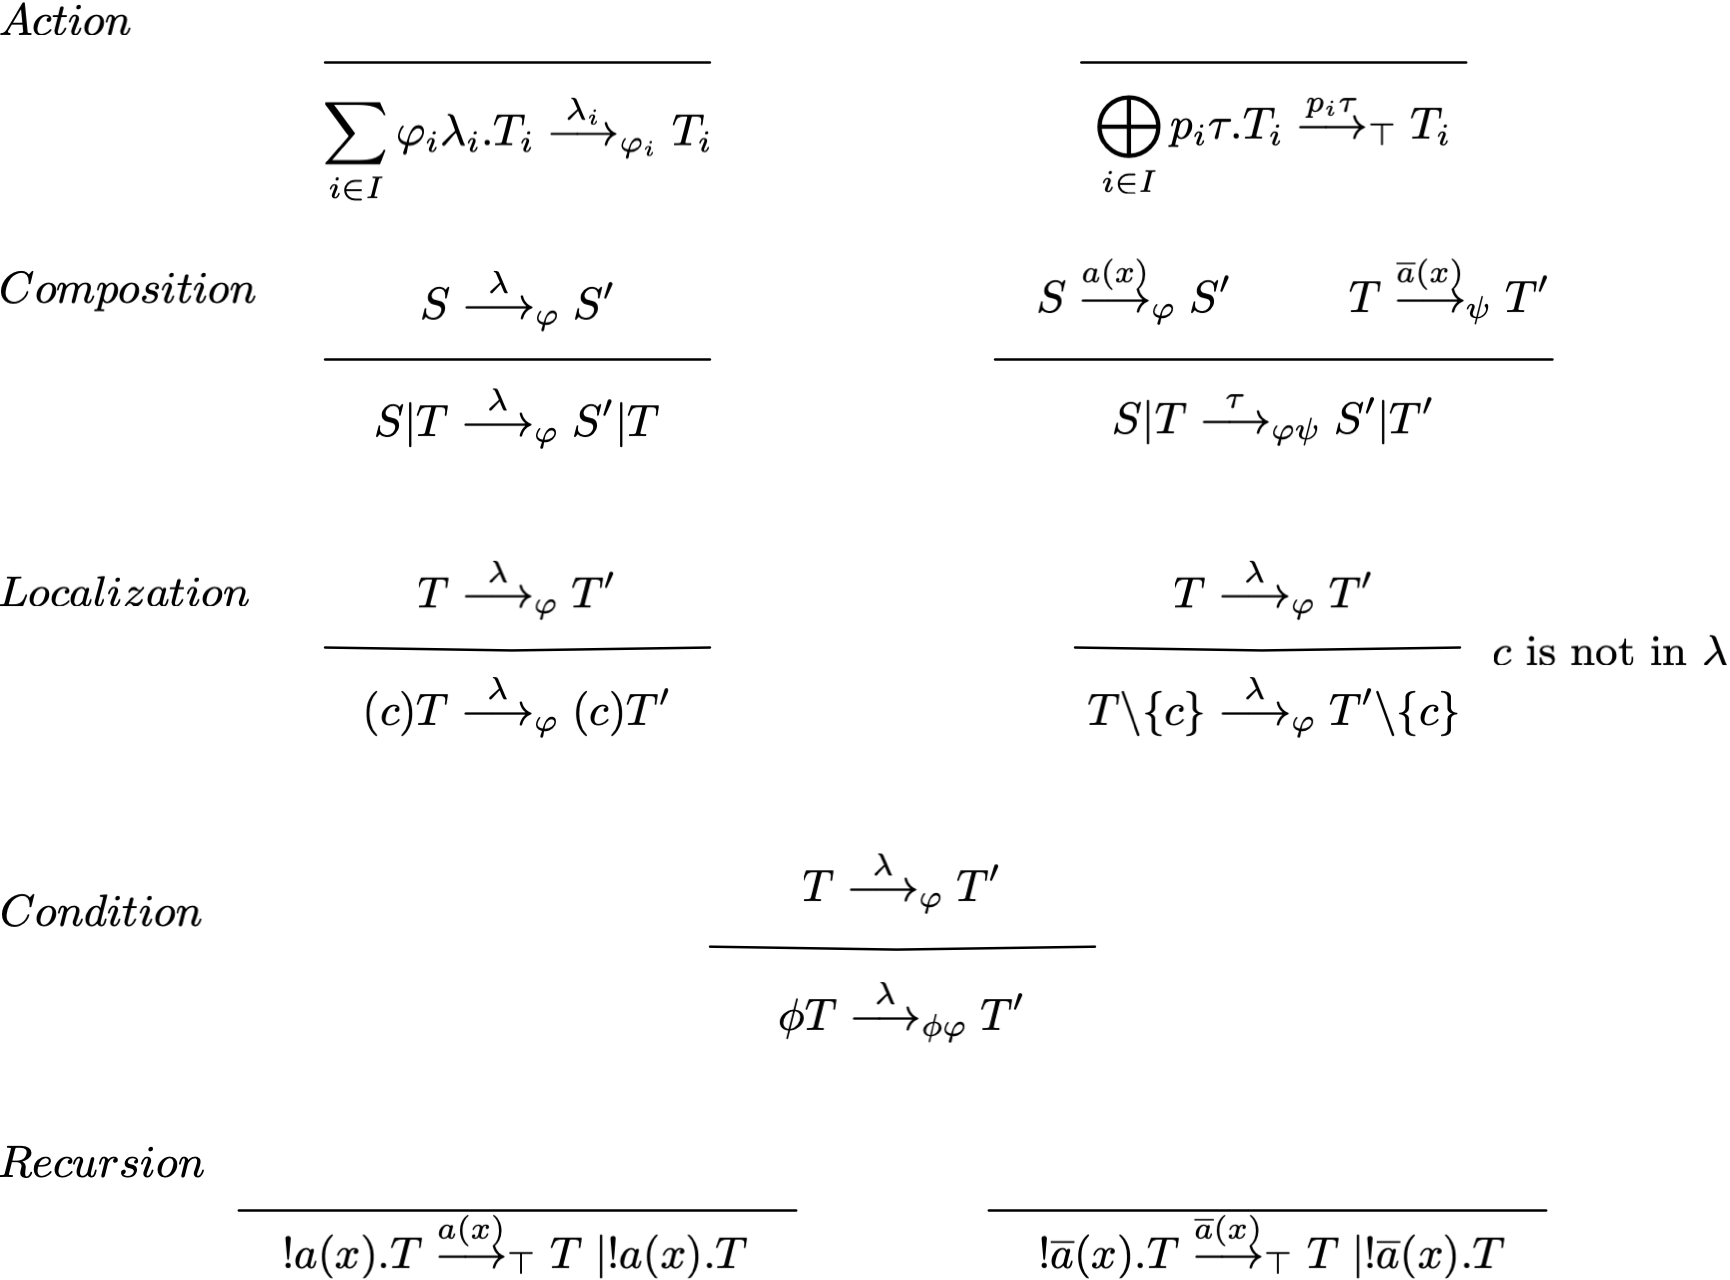
\includegraphics[width=14cm]{../figures/symbolic_sematic.png}
    \caption{\textbf{随机传值进程模型的符号迁移语义}}
    \label{fig_sematic}
\end{figure}

对于$\mathbb{VPC}_{\mathsf{Th}}$的前缀操作子的迁移规则:
$\sum_{i\in I} \varphi_i \lambda_i. T_i\stackrel{\lambda_i}{\rightarrow}_{\varphi_i} T_i$,
它本质上代表了非确定选择,
即作出$\varphi_i$条件下的$\lambda_i$动作到达$T_i$状态是非确定的,
我们可以通过Uniform Approach的方法将它扩展为一个概率性选择,
即在概率$p_i$下会作出$\varphi_i$条件下的$\lambda_i$动作:
$\bigoplus_{i\in I} p_i\tau.\varphi_i \lambda_i. T_i\stackrel{p_i\tau}{\rightarrow}_{\top}\stackrel{\lambda_i}{\rightarrow}_{\varphi_i} T_i$。
它的语义为:在概率$p_i$下,我们会经过一个内部$\tau$操作到达一个$\mathbb{RVPC}_{\mathsf{Th}}$状态:
$\varphi_i\lambda_i.T_i$,
若$\mathsf{Th}\vdash \varphi_i$(即一阶理论$\mathsf{Th}$下,$\varphi_i$为真),
则我们可以经过$\lambda_i$操作到达$\mathbb{RVPC}_{\mathsf{Th}}$状态$T_i$, 
其中$\lambda_i \in \{a(x),\bar{a}(x)\mid a\in \mathcal{N}, x\in \mathsf{V}_\Sigma, t\in \mathsf{T}_\Sigma\}\cup \{\tau\}$。

$\mathbb{RVPC}_{\mathsf{Th}}$在$\mathbb{VPC}_{\mathsf{Th}}$的基础上扩展了前缀操作:$p\tau.$,
其中$p\in (0,1)$。
类似$A=\tau.B$的$\mathbb{RVPC}_{\mathsf{Th}}$项,
我们可以认为$A\stackrel{1\tau}{\rightarrow}_{\top} B$,
这时也满足$A=\bigoplus_{i\in I} p_i\tau.A_i$的定义,
此时$I=\{1\},p_1=1,A_1=B$。
若将$\mathbb{VPC}_{\mathsf{Th}}$中的此类内部操作同样看待,
我们可以得出推论~\ref{co:vpc}。
\begin{corollary}\label{co:vpc}
   $\mathbb{VPC}_{\mathsf{Th}}$是一种特殊的$\mathbb{RVPC}_{\mathsf{Th}}$。
\end{corollary}

\section{随机传值进程模型中的互模拟关系}

\subsection{互模拟关系与观察等价性}\label{ch:bisimulation}

   程序理论的基本问题是进程的等价性。
   等价关系定义为:设$R$是非空集合$A$上的二元关系,
   若$R$是自反的、对称的、传递的,则称$R$是$A$上的等价关系。
   研究等价关系的目的在于将集合中的元素进行分类,选取每类的代表元素来降低问题的复杂度,如软件测试时,可利用等价类来选择测试用例\cite{Equiv}。
   对通信并发系统程序等价的定义和验证,现在已有很多研究。
   在提出CCS时MILNER R提出了\textit{观察等价(observation equivalence)}与\textit{弱互模拟(weak bisimulation)}\cite{Milner_CCS}。
   van GLABBEEK R和WEIJLAND W提出的\textit{分支互模拟(branching bisimulation)}\cite{Branching_1, Branching_2}也是十分著名的研究。

   对于概率模型的等价性,目前有对全概率进程模型,即概率选择代替非确定性选择的进程模型的弱互模拟及分支互模拟的研究\cite{全概率的弱互模拟和分支互模拟},
   仅适用于有限状态的概率进程模型的研究\cite{有限状态_1,有限状态_2}等。
   Uniform Approach在分支互模拟\cite{Branching_1, Branching_2}的基础上给出了
   RCCS分支互模拟关系的定义,以及等价关系同余性的证明。
   
   Uniform Approach中RCCS的分支互模拟涉及等价集的概念,我们首先看CCS等价集的定义:
   \begin{definition}
      若二元关系$\mathcal{E}$是$\mathcal{P}_{CCS}$上的等价关系。
      $A$关于等价关系$\mathcal{E}$的等价集写作$[A]_{\mathcal{E}}$,
      $A\in [A]_{\mathcal{E}}$,若$(A,B)\in \mathcal{E}$,
      有$B\in [A]_{\mathcal{E}}$。
      我们用$\mathcal{P}_{CCS}/\mathcal{E}$表示所有$\mathcal{P}_{CCS}$关于$\mathcal{E}$的等价集的集合。
   \end{definition}
   $\mathcal{P}_{RCCS}$,$\mathcal{T}_{\mathbb{VPC}_{\mathsf{Th}}}$,$\mathcal{T}_{\mathbb{RVPC}_{\mathsf{Th}}}$上的等价集的定义都是相似的,因此不做赘述。

   RCCS的分支互模拟是CCS分支互模拟的扩展,我们首先来看CCS的分支互模拟。
   $\mathcal{P}_{CCS}$上的分支互模拟的定义如下,其中内部操作$\tau$带来的状态迁移可以称为\textit{静态迁移},
   当$A\stackrel{\tau}{\rightarrow}A'\mathcal{E}A$时,我们可以写为$A\stackrel{\tau}{\rightarrow}_{\mathcal{E}}A'$,在Uniform Approach中,这种动作称为\textit{状态保持的静态迁移(state-preserving silent transition)},
   对应的若$A\stackrel{\tau}{\rightarrow}A'\notin [A]_{\mathcal{E}}$,称为\textit{状态改变的静态迁移}。
   $\Rightarrow_{\mathcal{E}}$为$\stackrel{\tau}{\rightarrow}_{\mathcal{E}}$的闭包。
   \begin{definition}
      $\mathcal{E}$是$\mathcal{P}_{CCS}$上的等价关系,
      若对于任意动作$l,l\neq \tau$和任意等价集$\mathcal{C}\in \mathcal{P}_{CCS}/\mathcal{E}, \mathcal{C}\neq [A]_{\mathcal{E}}$,
      满足若$B\mathcal{E}A\Rightarrow_{\mathcal{E}}\stackrel{l}{\rightarrow}\mathcal{C}$,则$B\Rightarrow_{\mathcal{E}}\stackrel{l}{\rightarrow}\mathcal{C}$,
      称$\mathcal{E}$是$\mathcal{P}_{CCS}$上的分支互模拟关系。
   \end{definition}

   考虑到RCCS在CCS的基础上增加了概率选择,
   状态保持的静态迁移在$A\stackrel{\tau}{\rightarrow}A'\mathcal{E}A$的基础上新增了
   $A\stackrel{p\tau}{\rightarrow} A'\mathcal{E}A,0<p<1$的可能,
   为了用类似$\Rightarrow_{\mathcal{E}}$的方式表示这种静态迁移,
   Uniform Approach提出了\textit{等价树(Epsilon Tree)}的概念[cite],
   将概率选择作为树的分支,节点$A$的关于等价关系$\mathcal{E}$的等价树上的任意节点$N\in [A]_{\mathcal{E}}$。
   同时,Uniform Approach定义了两种迁移:$l$-transition和$q$-transition,
   分别表示等价树上的节点迁移到其他等价集动作和概率。

   \begin{definition}[$l$-迁移($l$-transition)]
      $A\in \mathcal{P}_{RCCS}$,
      从$A$到$\mathcal{B}\in \mathcal{P}_{RCCS}/\mathcal{E},\mathcal{B}\neq [A]_{\mathcal{E}}$的
      $l$-迁移表示$A$关于等价关系$\mathcal{E}$的等价树上的每一个叶子结点$L$,
      存在$L\stackrel{l}{\rightarrow}L'\in\mathcal{B},l\neq \tau$,写作$A\rightsquigarrow_{\mathcal{E}}\stackrel{l}{\rightarrow}\mathcal{B}$。
   \end{definition}

   \begin{definition}[$q$-迁移($q$-transition)]
      $A\in \mathcal{P}_{RCCS}$,$\mathcal{E}$为$\mathcal{P}_{RCCS}$上的等价关系,
      $L$为$A$关于等价关系$\mathcal{E}$的等价树上的每一个叶子结点,
      $\mathcal{B}\in \mathcal{P}_{RCCS}/\mathcal{E}, \mathcal{B}\neq [A]_{\mathcal{E}}$。

      定义$\mathsf{P}(L\stackrel{\coprod_{i\in[k]}p_i\tau}{\longrightarrow}\mathcal{B})=\sum \{p_i|L\stackrel{p_i\tau}{\longrightarrow}L_i\in \mathcal{B}\wedge i\in I\}$。
      
      定义$\mathsf{P}_{\mathcal{E}}(L\stackrel{\coprod_{i\in[k]}p_i\tau}{\longrightarrow}\mathcal{B})=\mathsf{P}(L\stackrel{\coprod_{i\in[k]}p_i\tau}{\longrightarrow}\mathcal{B})/(1-\mathsf{P}(L\stackrel{\coprod_{i\in[k]}p_i\tau}{\longrightarrow}[A]_{\mathcal{E}}))$。

      当$\mathsf{P}_{\mathcal{E}}(L\stackrel{\coprod_{i\in[k]}p_i\tau}{\longrightarrow}\mathcal{B})=q$时,
      记为$A\rightsquigarrow_{\mathcal{E}}\stackrel{q}{\rightarrow}\mathcal{B}$,即$q$-迁移。
   \end{definition}

   现在我们终于可以引入Uniform Approach中定义的RCCS的分支互模拟关系了!

   \begin{definition}
      当$\mathcal{P}_{RCCS}$上的等价关系$\mathcal{E}$满足:
      \begin{itemize}
         \item {
            若$B\mathcal{E}A\rightsquigarrow_{\mathcal{E}}\stackrel{l}{\rightarrow}\mathcal{C}\in \mathcal{P}_{RCCS}/\mathcal{E}, l\neq \tau \wedge \mathcal{C}\neq [A]_{\mathcal{E}}$,则$B\rightsquigarrow_{\mathcal{E}}\stackrel{l}{\rightarrow}\mathcal{C}$。
         }
         \item {
            若$B\mathcal{E}A\rightsquigarrow_{\mathcal{E}}\stackrel{q}{\rightarrow}\mathcal{C}\in \mathcal{P}_{RCCS}/\mathcal{E}, l\neq \tau \wedge \mathcal{C}\neq [A]_{\mathcal{E}}$,则$B\rightsquigarrow_{\mathcal{E}}\stackrel{q}{\rightarrow}\mathcal{C}$。
         }
      \end{itemize}
      则等价关系$\mathcal{E}$是分支互模拟关系。
   \end{definition}

   对于传值进程模型,由于条件操作子的影响不能直接使用分支互模拟。
   在The Value-Passing Calculus中,FU Y提出了$\mathbb{VPC}_\mathsf{Th}$的符号互模拟。
   $\mathbb{VPC}_{\mathsf{Th}}$与CCS的区别主要体现在前缀操作子和条件操作子。
   对于前缀操作子,相似的定义互模拟关系是比较容易的,只需要保证通道一致、值一致即可。
   而条件操作子给互模拟的定义带来了麻烦,比如:
   $A=\overline{a}(0).S$和$B=((x=0) \overline{a}(0).S|\urcorner (x=0) \overline{a}(0).S)$在观察上应该是一致的,
   这就要求$B$的两个操作:$B\stackrel{\overline{a}(0)}{\longrightarrow}_{x=0} S$和$B\stackrel{\overline{a}(0)}{\longrightarrow}_{\urcorner (x=0)} S$共同模拟$A\stackrel{\overline{a}(0)}{\longrightarrow}_{\top} S$。
   为解决这一问题,The Value-Passing Calculus提出了符号互模拟:
   \begin{definition}[符号互模拟]\label{def:symbolic_bisimulation}
      $\mathcal{E}$是一个$\mathcal{T}_{\mathbb{VPC}_{\mathsf{Th}}}$上的二元对称关系,
      当$A\mathcal{E}B$满足下列条件时,称$\mathcal{E}$是一个符号互模拟关系:
      \begin{itemize}
         \item {
            若$A\stackrel{\tau}{\rightarrow}_{\varphi} A'$,则存在$\varphi$的划分$\{\varphi_i\}_{i\in I}$和集合$\{B\Rightarrow_{\psi_i} B_i\}_{i\in I}$,
            对于$\forall i\in I$,$\mathsf{Th}\vdash \varphi_i\Rightarrow \psi_i\wedge \varphi_i A\mathcal{E} \varphi_i B_i$,
            且满足$\varphi_i A'\mathcal{E} \varphi_i B_i$或$B_i\stackrel{\tau}{\rightarrow}_{\psi_i'}B_i'\wedge \mathsf{Th}\vdash \varphi_i\Rightarrow \psi_i'\wedge \varphi_i A'\mathcal{E} \varphi_i B_i'$。
         }
         \item {
            若$A\stackrel{\overline{a}(t)}{\rightarrow}_{\varphi} A'$,则存在$\varphi$的划分$\{\varphi_i\}_{i\in I}$和集合$\{B\Rightarrow_{\psi_i}B_i\stackrel{\overline{a}(t_i)}{\rightarrow}_{\psi_i'}B_i'\}$,
            满足$\mathsf{Th}\vdash (\varphi_i\Rightarrow \psi_i\psi_i')\wedge (\varphi_i \Rightarrow t=t_i)$且$(\varphi_i A\mathcal{E}\varphi_i B_i)\wedge(\varphi_i A'\mathcal{E}\varphi_i B_i')$。
         }
         \item {
            若$A\stackrel{a(x)}{\rightarrow}_{\varphi} A'$,则存在$\varphi$的划分$\{\varphi_i\}_{i\in I}$和集合$\{B\Rightarrow_{\psi_i}B_i\stackrel{a(x)}{\rightarrow}_{\psi_i'}B_i'\}$,
            满足$\mathsf{Th}\vdash \varphi_i\Rightarrow \psi_i\psi_i'$且$(\varphi_i A\mathcal{E}\varphi_i B_i)\wedge(\varphi_i A'\mathcal{E}\varphi_i B_i')$。
         }
      \end{itemize}
      互模拟关系的全集记为$\approxeq_{\mathsf{Th}}^s$。
   \end{definition}

   根据符号互模拟的定义,我们可以解决前述条件操作子带来的麻烦,
   我们可以通过下面的例子证明这一点。
   \begin{example}
      证明$A=\overline{a}(0).S$和$B=((x=0) \overline{a}(0).S|\urcorner (x=0) \overline{a}(0).S)$是符号互模拟的。
   \end{example}
   \begin{proof}
      定义等价关系$\mathcal{E}=\{(A,B)\}\cup \equiv$,
      其中$\equiv$为绝对等价关系,
      题目等价于证明$\mathcal{E}$是一个符号互模拟关系。

      对于$A\stackrel{\overline{a}(0)}{\rightarrow}_{\top} S$,
      存在$\top$的划分$\{(x=0),\urcorner(x=0)\}$和集合
      $\{B\stackrel{\overline{a}(0)}{\longrightarrow}_{x=0}S, B\stackrel{\overline{a}(0)}{\longrightarrow}_{\urcorner(x=0)}S\}$,
      且$(x=0)S\mathcal{E}(x=0)S$。

      对于$B\stackrel{\overline{a}(0)}{\longrightarrow}_{x=0}S$,存在$A\stackrel{\overline{a}(0)}{\longrightarrow}_{x=0}S$与之符号互模拟。
      $B\stackrel{\overline{a}(0)}{\longrightarrow}_{\urcorner(x=0)}S$同理。
   \end{proof}

   \subsection{条件等价树}

   根据~\ref{ch:bisimulation}中定义~\ref{def:symbolic_bisimulation}中定义的$\mathbb{VPC}_{\mathsf{Th}}$的符号互模拟关系,
   我们观察$A(x)=(x\geq 5)\overline{a}(\mathsf{s}(x)).0)$和$A'(x)=(x\geq 3)\overline{a}(\mathsf{s}(x)).0$,
   根据$\mathbb{VPC}_\mathsf{Th}$的符号互模拟的定义,我们容易得到$A$和$A'$是不符号互模拟的,
   对于$A'(t)\stackrel{\overline{a}(\mathsf{s}(t))}{\longrightarrow}_{x\geq 3} 0$,
   因为$3<x<5$的这一部分动作是$A(x)$无法完成的,所以不存在$x\geq 3$的划分,
   使得$A(x)$可以给出一个迁移的集合来模拟整个$x\geq 3$。
   但反观$B(x)=(x>5)A(x),B'(x)=(x>5)A'(x)$,
   我们可以得到$B'(x)=((x>5)\wedge(x\geq 3))\overline{a}(\mathsf{s}(x)).0=(x>5)\overline{a}(\mathsf{s}(x)).0$,
   同理$B(x)=(x>5)\overline{a}(\mathsf{s}(x)).0$,
   $B(x),B'(x)$不仅是符号互模拟,甚至是绝对等价的。
   对于$(x>5)A(x)$和$(x>5)A'(x)$的这种关系,
   我们给出\textit{条件等价集}的定义,可以使等价集内部对某个条件透明:

   \begin{definition}[条件等价集]
     $A,A'\in \mathcal{T}_{\mathbb{RVPC}_{\mathsf{Th}}}$,$\mathcal{E}$是$\mathbb{RVPC}_{\mathsf{Th}}$上的等价关系,
     若$\varphi A \mathcal{E} \varphi A'$,则$A'\in [A]_{\varphi \mathcal{E}}$。
     $[A]_{\varphi \mathcal{E}}$称为等价关系$\mathcal{E}$在条件$\varphi$下包含$A$的等价集。 
     我们用$\mathcal{T}_{\mathbb{RVPC}_{\mathsf{Th}}}/\varphi \mathcal{E}$表示所有$\mathbb{RVPC}_{\mathsf{Th}}$关于布尔表达式$\varphi$和等价关系$\mathcal{E}$的条件等价集的集合。 
   \end{definition} 

   由于$\mathbb{VPC}_{\mathsf{Th}}$是特殊的$\mathbb{RVPC}_{\mathsf{Th}}$,
   条件等价集的定义同样适用$\mathbb{VPC}_{\mathsf{Th}}$。
   显然,$A'(x)\in [A(x)]_{(x>5)\mathcal{E}}$,其中$\mathcal{E}=\approxeq_{\mathsf{Th}}^s$。
   
   条件$\top$具有一定的特殊性:
   对于无条件的操作我们认为操作是在$\top$条件下执行的,
   因此$\top$可以看作是最强的条件。
   \begin{corollary}\label{co:condition0}
      $A,B\in \mathcal{T}_{\mathbb{VPC}_{\mathsf{Th}}}$,
      若$A\approxeq_{\mathsf{Th}}^s B$,
      则对布尔表达式$\varphi$,
      $\varphi A\approxeq_{\mathsf{Th}}^s\varphi B$。
   \end{corollary}
   \begin{proof}
      对于$A$可以执行的操作,$\varphi' A$也会有对应的版本:
      \begin{itemize}
         \item 若$A\stackrel{\tau}{\rightarrow}_{\varphi} A'$,则$\varphi' A\stackrel{\tau}{\rightarrow}_{\varphi' \varphi}A'$。
         \item 若$A\stackrel{a(x)}{\rightarrow}_{\varphi} A'$,则$\varphi' A\stackrel{a(x)}{\rightarrow}_{\varphi' \varphi} A'$。
         \item 若$A\stackrel{\overline{a}(t)}{\rightarrow}_{\varphi} A'$,则$\varphi' A\stackrel{\overline{a}(t)}{\rightarrow}_{\varphi' \varphi} A'$。
      \end{itemize}
      对$\varphi' A\stackrel{a(x)}{\rightarrow}_{\varphi'\varphi} A'$,
      根据$A\approxeq_{\mathsf{Th}}^sB$,我们知道存在$\varphi$的划分$\{\varphi_i\}_{i\in I}$和集合$\{B\Rightarrow_{\psi_i}B_i\stackrel{a(x)}{\rightarrow}_{\psi_i'}B_i'\}_{i\in I}$,
      满足$\mathsf{Th}\vdash \varphi_i\Rightarrow \psi_i \psi_i' \wedge \varphi_i A\approxeq_{\mathsf{Th}}^s \varphi_i B_i \wedge \varphi_i A'\approxeq_{\mathsf{Th}}^s \varphi_i B_i'$。
      
      若要证明$\varphi' A\approxeq_{\mathsf{Th}}^s\varphi' B$,
      我们可以构造等价关系$\mathcal{S} = \{(\varphi'A,\varphi'B)|(A,B)\in \approxeq_{\mathsf{Th}}^s\}$,
      证明$\mathcal{S}$是符号互模拟的,其中$A,B$为任意$\mathcal{T}_{\mathbb{VPC}_{\mathsf{Th}}}$。

      通过$A\approxeq_{\mathsf{Th}}^sB$我们可以得到集合$\{\varphi'\varphi_i\}_{i\in I}$,
      对于任意$i,j$,由于$\varphi_i \wedge \varphi_j = \bot$,
      我们可以得到$(\varphi'\varphi_i) \wedge (\varphi'\varphi_j) = \bot$;
      又$\bigvee_{i\in I}\varphi_i = \varphi$,$\bigvee_{i\in I}\varphi'\varphi_i = \varphi'\varphi$,
      因此$\{\varphi'\varphi_i\}_{i\in I}$为$\varphi'\varphi$的划分。
      我们还可以得到集合$\{\varphi'B\Rightarrow_{\varphi'\psi_i}B_i\stackrel{a(x)}{\rightarrow}_{\psi_i'} B_i'\}$,
      满足$\mathsf{Th}\vdash \varphi'\varphi_i\Rightarrow \varphi'\psi_i\psi_i'$,
      而$(\varphi'\varphi_i A, \varphi'\varphi_i B_i),(\varphi'\varphi_i A', \varphi'\varphi_i B_i')\in \mathcal{S}$,
      因此我们可以用$\{\varphi'B\Rightarrow_{\varphi'\psi_i}B_i\stackrel{a(x)}{\rightarrow}_{\psi_i'} B_i'\}$模拟$\varphi' A\stackrel{a(x)}{\rightarrow}_{\varphi'\varphi} A'$。

      对称的一边和其他两种情况的证明是相似的。
   \end{proof}

   \begin{corollary}\label{co:all}
      $A,B\in \mathbb{RVPC}_{\mathsf{Th}}$,$\mathcal{E}$是$\mathbb{RVPC}_{\mathsf{Th}}$上的等价关系,
      $\varphi$是任意布尔表达式,
      若$B\in [A]_{\mathcal{E}}$,则$B\in [A]_{\varphi \mathcal{E}}$。
   \end{corollary}
   
   推论~\ref{co:all}可以简单理解为:一个$\mathbb{RVPC}_{\mathsf{Th}}$项在任意条件下成立的等价集是所有条件等价集的交集。
   我们也可以给出一个简单的证明。
   \begin{proof}
      $A,B\in \mathcal{T}_{\mathbb{RVPC}_{\mathsf{Th}}}$,
      $fv(\varphi)$为$\varphi$中的自由变元的集合,
      $V$为$fv(\varphi)$的全部取值的集合,
      对于$fv(\varphi)$的每一个赋值$v\in V$,
      我们可以得到一个无自由变元的布尔表达式$\varphi_v$:
      \begin{itemize}
         \item {
            若$\mathsf{Th}\vdash \varphi_v$,$\varphi_vA=A\mathcal{E}B=\varphi_v B$。
         }
         \item {
            若$\mathsf{Th}\not\vdash \varphi_v$,$\varphi_v A=0=\varphi_v B$。
         }
      \end{itemize}
   \end{proof}

   将$\top$推广到其他布尔表达式,我们可以得到更为广泛的结论:

   \begin{corollary}\label{co:condition}
      $A,B\in \mathcal{T}_{\mathbb{VPC}_{\mathsf{Th}}}$,
      若$\varphi A\approxeq_{\mathsf{Th}}^s \varphi B$,
      则对布尔表达式$\varphi',\mathsf{Th}\vdash \varphi'\Rightarrow \varphi$,
      $\varphi' A\approxeq_{\mathsf{Th}}^s\varphi' B$。
   \end{corollary}

   \begin{corollary}\label{co:all_1}
      $A,B\in \mathbb{RVPC}_{\mathsf{Th}}$,$\mathcal{E}$是$\mathbb{RVPC}_{\mathsf{Th}}$上的等价关系,
      $\varphi$是任意布尔表达式,
      若$B\in [A]_{\varphi\mathcal{E}}$,
      则对于布尔表达式$\varphi',\mathsf{Th}\vdash\varphi'\Rightarrow \varphi$,
      $B\in [A]_{\varphi' \mathcal{E}}$。
   \end{corollary}

   \begin{corollary}\label{co:superset}
      $L\in \mathcal{T}_{\mathbb{RVPC}_{\mathsf{Th}}}$,
      $L$关于布尔表达式$\varphi$和等价关系$\mathcal{E}$的等价集为$\mathcal{C}=[L]_{\varphi\mathcal{E}}$,
      对任意$\mathsf{Th}\vdash \varphi'\Rightarrow\varphi$,
      $L$关于$\varphi'\mathcal{E}$的等价集$[L]_{\varphi'\mathcal{E}}$是$\mathcal{C}$的超集,
      可以将$[L]_{\varphi'\mathcal{E}}$记为$[\mathcal{C}]_{\varphi'\mathcal{E}}$。
   \end{corollary}
   推论~\ref{co:superset}可以由推论~\ref{co:all_1}得出。

   定义~\ref{def:symbolic_bisimulation}给出了$\mathbb{VPC}_{\mathsf{Th}}$的互模拟的定义,
   观察定义~\ref{def:symbolic_bisimulation}中的$A\stackrel{a(x)}{\longrightarrow}_{\varphi} A'$,
   我们用$\{B\Rightarrow_{\psi_i}B'_i\stackrel{a(x)}{\longrightarrow}_{\psi'_i}B_i'\}$模拟,
   其中$(\varphi_i A\mathcal{E}\varphi_i B_i)\wedge(\varphi_i A'\mathcal{E}\varphi_i B_i')$,
   根据条件等价集的定义,我们可以得到$B_i\in [A]_{\varphi\mathcal{E}}$,$B_i'\in [A']_{\varphi \mathcal{E}}$,
   由于$B_i \approxeq_{\mathsf{Th}}^s A$,$B_i\approxeq_{\mathsf{Th}}^s B$,那么$B\Rightarrow_{\psi_i}B_i\in[B]_{\varphi\mathcal{E}}$实际上也是\textit{状态保持的静态迁移}。

   对于我们概率扩展后的$\mathbb{RVPC}_{\mathsf{Th}}$,
   对上述例子状态保持静态迁移多了$B\stackrel{q\tau}{\rightarrow}_{\psi_i} B_i$
   的情况,其中$q\in(0,1)$,表示\textit{概率的状态保持的静态迁移}。
   我们希望可以找到$\mathbb{RVPC}_{\mathsf{Th}}$中类似$\Rightarrow$的方式来表达这种状态保持的静态迁移。
   我们可以使用Uniform Approach中等价树的方法来刻画这种状态保持的静态迁移,
   在$\mathbb{RVPC}_{\mathsf{Th}}$中称为\textit{条件等价树}。

   在定义条件等价树之前,我们首先关注一种条件无关的静态迁移树:
\begin{definition}[静态迁移树]
   \label{def:silent_tree}
   若$A\in \mathcal{T}_{\mathbb{RVPC}_{\mathsf{Th}}}$,
   $A$的静态迁移树$t$满足如下定义:
   \begin{itemize}
   \item 每一个节点都被标记成$\mathcal{T}_{\mathbb{RVPC}_{\mathsf{Th}}}$的一个项,$A$是根节点。
   \item {
      节点间的边被标记成$(\varphi,p)$,其中$p\in(0,1]$,$\varphi$是一个布尔表达式。
      如果一条从$A'$到$A''$的有向边被标记成$(\varphi,p)$,表示$A'\stackrel{p\tau}{\rightarrow}_{\varphi} A''$。
   }
   \end{itemize}
\end{definition}

静态迁移树包含了\textit{状态改变的静态迁移}和\textit{状态保持的静态迁移},
条件等价树需要对特定条件下的状态改变的静态迁移进行剪枝:

\begin{definition}[条件等价树]
   $\varphi$是一个布尔表达式,$\mathcal{E}$是$\mathcal{T}_{\mathbb{RVPC}_{\mathsf{Th}}}$上的等价关系,
   $A\in \mathcal{T}_{\mathbb{RVPC}_{\mathsf{Th}}}$,
   当下列条件成立时,$A$的静态迁移树$t$称为是一个关于$\varphi\mathcal{E}$的条件等价树($\varphi \mathcal{E}$-tree) ,记作$t^A_{\varphi \mathcal{E}}$。
\begin{itemize}
   \item[(1)] $t$上的所有节点$N$,$N\in [A]_{\varphi \mathcal{E}}$,并被重新标记为$\varphi N$。
   \item[(2)] {
   若$t$的边被标记为$(\psi, q)$,则$\mathsf{Th}\vdash \varphi\Rightarrow \psi$。
   }
   \item[(3)] {
         若$B,B'$是$t$上的节点,
         $B\stackrel{(\psi,q)}{\rightarrow}B',q\in (0,1)$,
         则存在$B\stackrel{\coprod_{i\in [k]}}{\longrightarrow}_{\psi} \coprod_{i\in [k]} B_i$,
         $B_i,i\in [k]$是$t$上的节点,
         且$B$有且仅有$B_1,\dots, B_k$这$k$个儿子节点,
         且根据(2),有$\mathsf{Th}\vdash \varphi\Rightarrow \psi$。
   }
   \item[(4)] {
      若$B,B'$是$t$上的节点,
      $B\stackrel{(\psi,1)}{\rightarrow}B'$,
      则有$B\stackrel{\tau}{\rightarrow}_{\psi}B'$且$B$有且仅有$B'$一个儿子节点,
      且根据(2),有$\mathsf{Th}\vdash \varphi\Rightarrow \psi$。
   }
\end{itemize}
\end{definition}

条件等价树实质上是\textit{概率的状态保持的静态迁移}。

从定义上看条件等价树的定义比较抽象,我们可以看几个简单有趣的例子:

\begin{example}\label{eg:conditional}
   $A(x)=(x>5)(\frac{1}{2}\tau.B(x)\oplus\frac{1}{2}\tau.C(x))|(x\leq 5)(\frac{1}{3}\tau.B(x)\oplus\frac{2}{3}\tau.C(x))$。
   若$[A(x)]_{\mathcal{E}}=[B(x)]_{\mathcal{E}}=[C(x)]_{\mathcal{E}}$,
   我们可以得到$A(x)$的静态迁移树如图\ref{fig:eg_condition},$A(x)$关于$(x>7)\mathcal{E}$的条件等价树如图\ref{fig:eg_condition2}。

\begin{figure}[!htp]
   \begin{minipage}{0.6\textwidth}
   \centering
   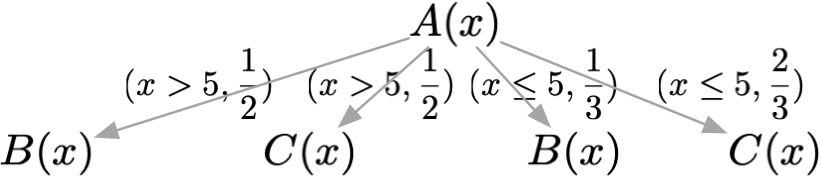
\includegraphics[width=8cm]{../figures/example_condition.png}
   \caption{}
  \label{fig:eg_condition}
\end{minipage}\hfill
\begin{minipage}{0.45\textwidth}
   \centering
   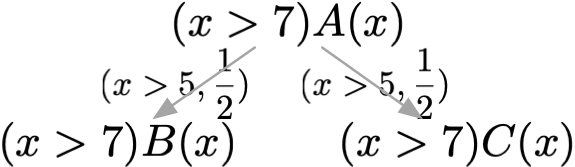
\includegraphics[width=5cm]{../figures/example_condition2.png}
   \caption{}
   \label{fig:eg_condition2}
\end{minipage}
 \end{figure}
\end{example}
\begin{example}
   $H(x)\stackrel{def}{=}(x\leq 3)(\frac{1}{3}\tau.(x\leq 1)G(x)\oplus\frac{1}{3}\tau.(x\leq 2)G(x)\oplus\frac{1}{3}\tau.(x\leq 3)G(x))$

   $[H(x)]_{\mathcal{E}_1} = [G(x)]_{\mathcal{E}_1}$,$H(x),G(x)\in \mathbb{RVPC}_{\mathsf{Th}}$,其中$\mathsf{Th}=\mathsf{PA}$[cite]。

   $H(x)$的静态迁移树如图~\ref{fig_eg0_1},它包含了$H(x)$所有的静态迁移。
   \begin{figure}[!htp]
      \begin{minipage}{0.6\textwidth}
         \centering
         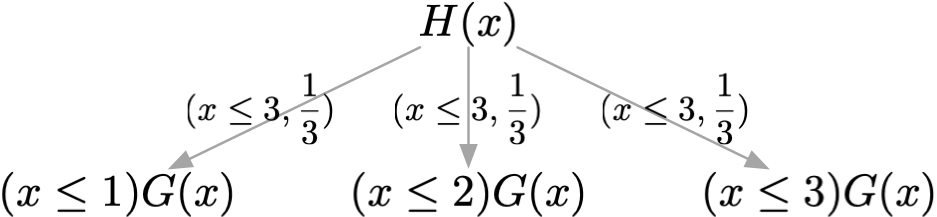
\includegraphics[width=8cm]{../figures/example0_1.png}
         \caption[]{}
         \label{fig_eg0_1}
   \end{minipage}\hfill
   \begin{minipage}{0.45\textwidth}
      \centering
      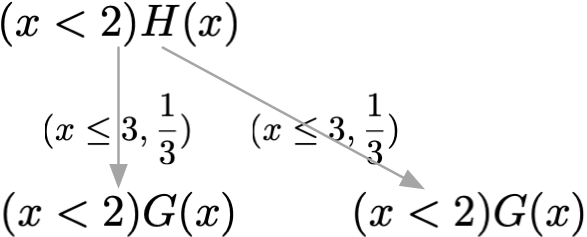
\includegraphics[width=5cm]{../figures/example0_2.png}
      \caption[]{}
       \label{fig_eg0_2}
   \end{minipage}
    \end{figure}

   因为$\mathsf{Th}\vdash \top \not\Rightarrow (x\leq 3)$,
   $H(x)$的$\top\mathcal{E}_1$-tree只有一个根节点$H(x)$。

   同理,$H(x)$的$(x>3)\mathcal{E}_1$-tree只有一个根节点$H(x)$。

   $H(x)$的$(x<2)\mathcal{E}_1$-tree如图~\ref{fig_eg0_2},
   其中$\mathsf{Th}\vdash (x<2)\Rightarrow (x\leq 3)$,
   由于$(x<2)\wedge(x\leq 2)G(x) = (x<2)G(x)$,$G(x)\in[H(x)]_{\mathcal{E}_1}$,
   根据推论~\ref{co:all},$(x\leq 2)G(x)\in [H(x)]_{(x<2)\mathcal{E}_1}$。
   另一个分支同理。此时$(x<2)H(x)\stackrel{\frac{2}{3}\tau}{\rightarrow}_{\top}[(x<2)G(x)]_{(x<2)\mathcal{E_1}}$,
   因此在条件树内部,我们可以将节点和边都视为状态无关。

\end{example}
\begin{example}\label{eg:1}
      假设我们有一个不太行的下课铃系统,每一时刻它坏掉的可能性是$\frac{1}{2}$,可以通过内部自动校准系统(静态迁移:$\tau$操作)修复,
      它的内部有一个计时器,每隔定长时间($\tau$操作)就会从$a$通道广播录好的一段下课铃,
      录好的下课铃可以用变元$x$表示。
      这个下课铃系统可以被抽象为一个$\mathbb{RVPC}_{\mathsf{Th}}$,其中$\mathsf{Th}$可以认为是$\mathsf{PA}$,
      我们可以用$G(x)$来表示这个系统:
      $$G(x)\stackrel{def}{=}\mu X.(\frac{1}{2}\tau.X\oplus \frac{1}{2}\tau.\overline{a}(x).X)$$
      $G(x)$在$\mathcal{E}_2$的等价集$[G(x)]_{\top\mathcal{E}_2} = [\overline{a}(x).G(x)]_{\top\mathcal{E}_2}$。
      $G(x)$的$\top \mathcal{E}_2$-tree如图~\ref{fig_eg1}。
      \begin{figure}[!htbp]
         \small
         \centering
         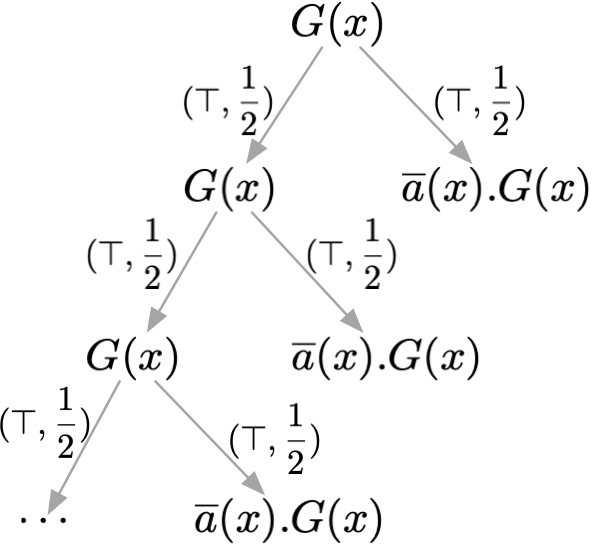
\includegraphics[width=5cm]{../figures/example1.png}
         \caption[]{} 
         \label{fig_eg1}
      \end{figure}
\end{example}
\begin{example}\label{eg:2}
   假设例~\ref{eg:1}的下课铃系统经过岁月的磨练,年久失修,
   每自动校准一次音量就会减弱,我们用变元$y$来表示音量,
   音量必须满足$y>1$才可以播放,
   当$y\leq 0$时下课铃系统音量就无法减弱了。
   为了方便建模,我们用$\mathsf{p}(x)=x-1$来表示这种音量减弱。
   校长出于节约经费的考虑,只要下课铃还能在他办公室听见($y>3$)就可以继续使用,
   现在的下课铃系统依然是一个$\mathbb{RVPC}_{\mathsf{Th}}$,
   我们可以用修改的$G'(x,y)$来表示这个系统:
   $$G'(x,y)\stackrel{def}{=}(y>3)(\frac{1}{2}\tau.((y>0)\tau.G'(x,\mathsf{p}(y))|\urcorner (y>0)\tau.G'(x,y))\oplus \frac{1}{2}\tau.((y>1)\overline{a}(x).G'(x,y)))$$
   $G'(x,y)$在$(y>3)\mathcal{E}_3$的等价集$[G'(x,y)]_{(y>3)\mathcal{E_3}}=[G'(x,y')]_{(y'>3)\mathcal{E_3}}=[\overline{a}(x).G'(x,y'')]_{(y''>3)\mathcal{E_3}}$,其中$y,y',y''$不一定相等。

   $G'(x,y)$的$(y>3)\mathcal{E}_3$-tree如图~\ref{fig_eg2}。
   \begin{figure}[!htbp]
      \small
      \centering
      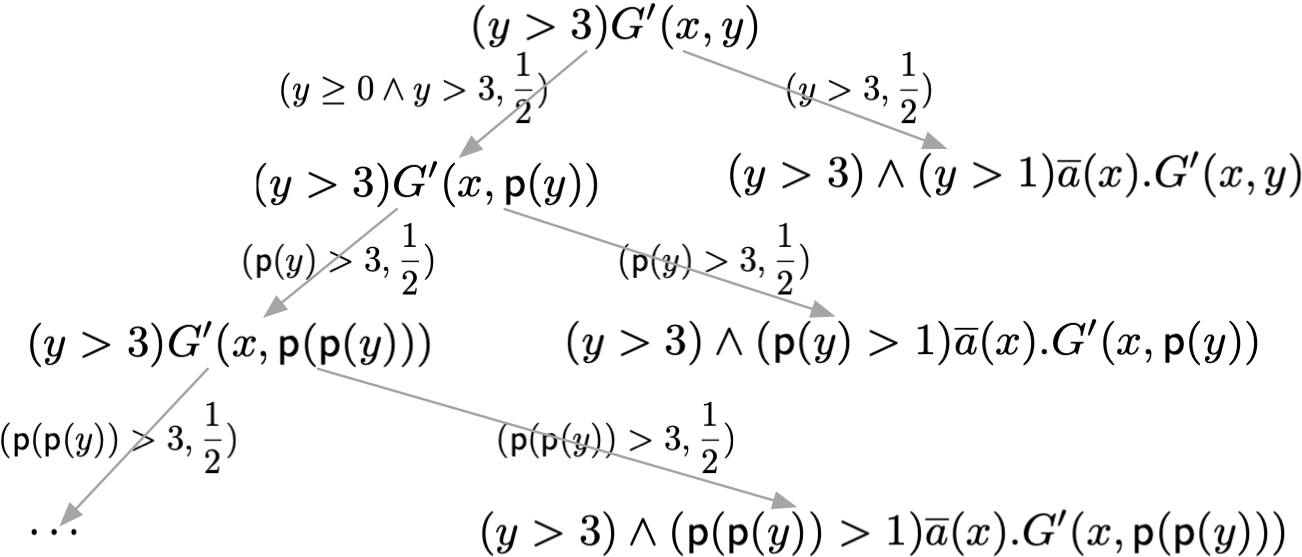
\includegraphics[width=11cm]{../figures/example2.png}
      \caption[]{} 
      \label{fig_eg2}
   \end{figure}

\end{example}

\subsection{随机传值进程模型的符号互模拟}\label{ch:symbolic_bisimulation}
定义了\textit{概率的状态保持的静态迁移},
我们现在可以用Uniform Approach的方法得到$\mathbb{RVPC}_{\mathsf{Th}}$的符号互模拟。
我们首先需要定义随机传值进程模型条件版的$l$-迁移和$q$-迁移。

\begin{definition}[条件$l$-迁移($\varphi l$-transition)]
   $A\in \mathcal{T}_{\mathbb{RVPC}_{\mathsf{Th}}}, \mathcal{B}\in \mathcal{T}_{\mathbb{RVPC}_{\mathsf{Th}}}/\varphi'\mathcal{E}\backslash \{[A]_{\varphi'\mathcal{E}}\}$,
   其中$\varphi'$是一个布尔表达式,$\mathcal{E}$是$\mathcal{T}_{\mathbb{RVPC}_{\mathsf{Th}}}$上的等价关系,
   若$A$的条件等价树$t_{\varphi' \mathcal{E}}^A$的所有叶子结点$L$,
   存在$L\stackrel{l}{\rightarrow}_{\varphi} L'\in \mathcal{B},l\neq \tau$,
   称为$\varphi'$条件下$A$到$\mathcal{B}$的$\varphi l$-迁移,记作$A\rightsquigarrow_{\varphi'\mathcal{E}}\stackrel{l}{\rightarrow}_{\varphi}\mathcal{B}$。
\end{definition}

\begin{definition}[条件$q$-迁移($\varphi q$-transition)]
   $A\in \mathcal{T}_{\mathbb{RVPC}_{\mathsf{Th}}},\mathcal{B}\in (\mathcal{T}_{\mathbb{RVPC}_{\mathsf{Th}}}/\varphi' \mathcal{E})\backslash \{[A]_{\varphi'\mathcal{E}}\}$,
   其中$\varphi'$是一个布尔表达式,$\mathcal{E}$是$\mathcal{T}_{\mathbb{RVPC}_{\mathsf{Th}}}$上的等价关系,
   对$t^A_{\varphi' \mathcal{E}}$的每一个叶子结点$L$和布尔表达式$\varphi$,
   若$L\stackrel{\coprod_{i\in I}p_i\tau}{\longrightarrow}_{\coprod_{i\in I}\psi_i} \coprod_{i\in [k]}L_i$,
$i\in I, L_i\in \mathcal{B}$,且$\mathsf{Th}\vdash \varphi \Rightarrow \psi_i$:

定义$\mathsf{P}_\varphi(L\stackrel{\coprod_{i\in I}p_i\tau}{\longrightarrow}_{\coprod_{i\in I}\psi_i}\mathcal{B}) = \sum\{p_i\mid L\stackrel{p_i\tau}{\rightarrow}_{\psi_i} L_i\in\mathcal{B} \wedge i\in I \wedge \mathsf{Th}\vdash \varphi \Rightarrow \psi_i\}$。

定义$\mathsf{P}_{\varphi, \varphi' \mathcal{E}}(L\stackrel{\coprod_{i\in I}p_i\tau}{\longrightarrow}_{\coprod_{i\in I}\psi_i}\mathcal{B}) = \mathsf{P}_\varphi(L\stackrel{\coprod_{i\in I}p_i\tau}{\longrightarrow}_{\coprod_{i\in I}\psi_i}\mathcal{B})/(1-\mathsf{P}_\varphi(L\stackrel{\coprod_{i\in I}p_i\tau}{\longrightarrow}_{\coprod_{i\in I}\psi_i}[A]_{\varphi\mathcal{E}}))$。

当$\mathsf{P}_{\varphi,\varphi' \mathcal{E}}(L\stackrel{\coprod_{i\in I}p_i\tau}{\longrightarrow}_{\coprod_{i\in I}\psi_i}\mathcal{B})=q$时,
称$\varphi'$条件下$A$到$\mathcal{B}$存在$\varphi q$-迁移。写作$A\rightsquigarrow_{\varphi'\mathcal{E}} \stackrel{q}{\rightarrow}_{\varphi} \mathcal{B}$。
\end{definition}

符号互模拟实质上是保证$\mathcal{T}_{\mathbb{RVPC}_{\mathsf{Th}}}$上的等价关系满足条件$l$-迁移和条件$q$-迁移的互模拟。
\begin{definition}[符号互模拟]\label{def:rvpc_symbolic_bisimulation}
   $\mathcal{E}$是一个$\mathcal{T}_{RVPC}$上的二元对称关系,
当$A\mathcal{E}B$且满足下列条件时,称$\mathcal{E}$是一个符号互模拟(Symbolic Bisimulation):
\begin{itemize}
   \item {
      若$ A \rightsquigarrow_{\varphi \mathcal{E}}\stackrel{a(x)}{\rightarrow}_{\varphi} L\notin [A]_{\varphi \mathcal{E}}$,
      则存在$\varphi$的划分$\{\varphi_i\}_{i\in I}$,和集合$\{B\rightsquigarrow_{\varphi_i \mathcal{E}}\stackrel{a(x)}{\rightarrow}_{\psi_i} L'\in[L]_{\varphi_i\mathcal{E}}\}$,
      使得对$i\in I$,$\mathsf{Th}\vdash \varphi_i \Rightarrow \psi_i$。
   }
   \item {
      若$A \rightsquigarrow_{\varphi \mathcal{E}}\stackrel{\bar{a}(t)}{\rightarrow}_{\varphi} L\notin [A]_{\varphi\mathcal{E}}$,
      则存在$\varphi$的划分$\{\varphi_i\}_{i\in I}$,和集合$\{B\rightsquigarrow_{\varphi_i\mathcal{E}}\stackrel{\bar{a}(t_i)}{\rightarrow}_{\psi_i} L'\in [L]_{\varphi_i\mathcal{E}}\}$,
      使得对$i\in I$,$\mathsf{Th}\vdash (\varphi_i \Rightarrow \psi_i)\wedge (\varphi_i \Rightarrow (t=t_i))$。
   }
   \item {
      若$ A\rightsquigarrow_{\varphi\mathcal{E}} \stackrel{q}{\rightarrow}_{\varphi} \mathcal{C}\in \mathcal{T}/\mathcal{E}, \mathcal{C}\neq [A]_{\varphi \mathcal{E}}$,
      则存在$\varphi$的划分$\{\varphi_i\}_{i\in I}$,和集合$\{B\rightsquigarrow_{\varphi_i\mathcal{E}}\stackrel{q_i}{\rightarrow}_{\varphi_i} [\mathcal{C}]_{\varphi_i\mathcal{E}}\}$,
      使得$i\in I$,$q_i= q$。
   }
\end{itemize}
\end{definition}

如果RCCS的分支互模拟可以看作是用等价树模拟等价树,
$\mathbb{RVPC}_{\mathsf{Th}}$的符号互模拟可以看作是等价森林模拟等价树。
我们可以给出等价森林的递归定义。

\begin{definition}[条件等价森林]
   $A\in\mathcal{T}_{\mathbb{RVPC}_{\mathsf{Th}}}$,$\mathcal{E}$是$\mathcal{T}_{\mathbb{RVPC}_{\mathsf{Th}}}$上的等价关系,
   $\varphi$是一个布尔表达式,
   对于$\varphi$的一个划分$\{\varphi_i\}_{i\in I}$,
   $A$关于$\varphi\mathcal{E}$的条件等价森林有且仅有$A$关于$\varphi_i\mathcal{E}$的条件等价树或条件等价森林,$i\in I$。
\end{definition}

在证明$\mathcal{T}_{\mathbb{RVPC}_{\mathsf{Th}}}$的两项符号互模拟时,
我们通常可以构造一个含有该项的等价集,并证明该等价集是一个符号互模拟关系。
构建一个$\mathcal{T}_{\mathbb{RVPC}_{\mathsf{Th}}}$项的条件$l$-迁移和条件$q$-迁移时,
我们可以首先构建该项的\textit{静态迁移树}。

\begin{example}\label{eg:5}
   假设学校负责看管设备的老师发现例~\ref{eg:2}中的下课铃系统其实只有在$y\geq 5$时才能被所有教室的同学们听到,
   为了不违抗校长的决定又同时让同学们都听到下课铃,他决定当$(y<5)$时用自己的电脑通过$a$通道播放下课铃,
   这时校长以为下课铃系统被工人修好成例~\ref{eg:1}中的下课铃系统,决定一直使用这个下课铃。校长的感觉是错觉吗?

   此时,看管设备的老师和例~\ref{eg:2}中的下课铃系统依旧是一个$\mathbb{RVPC}_{\mathsf{Th}}$,
   我们可以用$G''(x,y)$来表示这个系统。

   $G''(x,y) = (\frac{1}{2}\tau.((y>0)\tau.G''(x,\mathsf{p}(y))|\urcorner (y>0)\tau.G''(x,y))\oplus \frac{1}{2}\tau.((y>1)\overline{a}(x).G''(x,y)|(y<5)\overline{a}(x).G''(x,y))$。

   我们只需要证明$G(x)$与$G''(x,y)$符号互模拟即可。
\end{example}
\begin{proof}
   构造等价集
   \begin{align*}
      \mathcal{S} &= \{(G(x),G''(x,y)),\\
      &(G(x),(y>0)\tau.G''(x,\mathsf{p}(y))|\urcorner (y>0)\tau.G''(x,y)),\\
      &(\overline{a}(x).G(x),(y>1)\overline{a}(x).G''(x,y)|(y<5)\overline{a}(x).G''(x,y)),\\
      &(G(t),G''(t,y))|t\in V\}
   \end{align*}
   其中$V$是$x$的取值范围。
   我们只需证明$\mathcal{S}$是一个符号互模拟关系即可。
   \begin{itemize}
      \item {
         $\overline{a}(x).G(x)$和$(y>1)\overline{a}(x).G''(x,y)|(y<5)\overline{a}(x).G''(x,y)$关于$(x=t)\mathcal{S}$的等价树只有一个根节点,
         由于不涉及概率,这里实际可以使用$\mathbb{VPC}_{\mathsf{Th}}$的符号互模拟证明,
         但由于$\mathbb{VPC}_{\mathsf{Th}}$是$\mathbb{RVPC}_{\mathsf{Th}}$的特例,
         此处依然可以使用$\mathbb{RVPC}_{\mathsf{Th}}$的符号互模拟证明。
         \begin{itemize}
            \item {
               对于$x$的每一个赋值$t\in V$,
               $\overline{a}(x).G(x)\rightsquigarrow_{(x=t)\mathcal{S}}\stackrel{\overline{a}(t)}{\longrightarrow}_{(x=t)}G(t)$。
               我们可以得到$(x=t)$的一个划分:$(x=t)=((y>1)\wedge (x=t))\vee ((y\leq 1)\wedge (x=t))$。
      
               这时存在集合
               $$\{(y>1)\overline{a}(x).G''(x,y)|(y<5)\overline{a}(x).G''(x,y)\rightsquigarrow_{(x=t)\wedge(y>1)\mathcal{S}}\stackrel{\overline{a}(t')}{\rightarrow}_{(y>1)}G''(t',y),$$
               $$(y>1)\overline{a}(x).G''(x,y)|(y<5)\overline{a}(x).G''(x,y)\rightsquigarrow_{(x=t)\wedge(y\leq 1)\mathcal{S}}\stackrel{\overline{a}(t')}{\rightarrow}_{(y<5)}G''(t',y)\}$$
               可以模拟上述操作,
               其中$\mathsf{Th}\vdash(x=1)\wedge(y\leq 1)\Rightarrow (y<5)$
               且$\mathsf{Th}\vdash (x=t)\wedge (y\leq 1)\Rightarrow (t=t')$,
               $G''(t,y)\in[G(t)]_{(x=t)\wedge(y\leq 1)\mathcal{S}}$。$(x=t)\wedge(y>1)$相同。
            }
            \item {
               对$x$的每一个赋值$t\in V$,
               $$(y>1)\overline{a}(x).G''(x,y)|(y<5)\overline{a}(x).G''(x,y)\rightsquigarrow_{(x=t)\wedge(y>1)\mathcal{S}}\stackrel{\overline{a}(t)}{\rightarrow}_{(x=t)\wedge(y>1)}G''(t,y)$$,
               
               存在集合$\{\overline{a}(x).G(x)\rightsquigarrow_{(x=t)(y>1)\mathcal{S}}\stackrel{\overline{a}(t')}{\longrightarrow}_{(x=t)}G(t')\}$
               可以模拟上述操作,其中$\mathsf{Th}\vdash ((x=t)\wedge (y>1))\Rightarrow (x=t) \wedge \mathsf{Th}\vdash ((x=t)\wedge (y>1))\Rightarrow t=t'$,$G(t)\in [G''(t,y)]_{(x=t)\wedge (y>1)\mathcal{S}}$。
               
               对$x$的每一个赋值$t\in V$,
               $$(y>1)\overline{a}(x).G''(x,y)|(y<5)\overline{a}(x).G''(x,y)\rightsquigarrow_{(x=t)\wedge(y<5)\mathcal{S}}\stackrel{\overline{a}(t)}{\rightarrow}_{(x=t)\wedge(y<5)}G''(t,y)$$,
               
               存在集合$\{\overline{a}(x).G(x)\rightsquigarrow_{(x=t)(y<5)\mathcal{S}}\stackrel{\overline{a}(t')}{\longrightarrow}_{(x=t)}G(t')\}$
               可以模拟上述操作,其中$\mathsf{Th}\vdash ((x=t)\wedge (y<5))\Rightarrow (x=t) \wedge\mathsf{Th}\vdash ((x=t)\wedge (y<5))\Rightarrow t=t'$,$G(t)\in [G''(t,y)]_{(x=t)\wedge (y<5)\mathcal{S}}$。
            }
         \end{itemize}
      }
      \item {
         $(G(t),(y>0)\tau.G''(x,\mathsf{p}(y))|\urcorner (y>0)\tau.G''(x,y))$的这一对等价关系也是常规的$\mathbb{VPC}_{\mathsf{Th}}$证明,此处不做赘述。
      }
      \item {
         $G(x)$的静态迁移树如图~\ref{fig_eg4_1},$G''(x,y)$的静态迁移树如图~\ref{fig_eg4_2}。
         \begin{figure}[!htbp]
            \caption[]{}
            \small
            \centering
            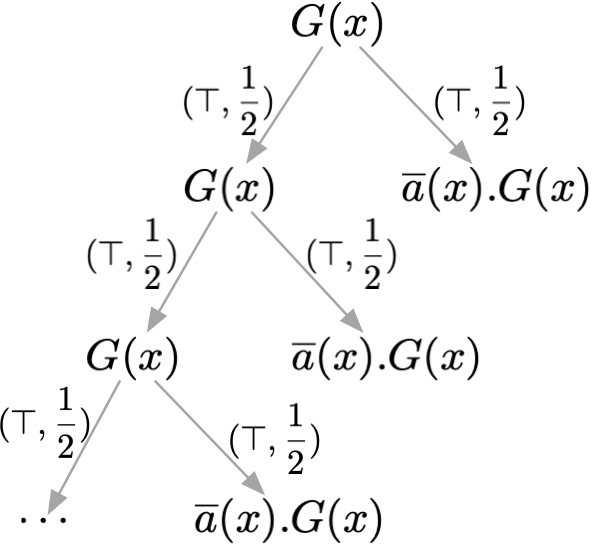
\includegraphics[width=5cm]{../figures/example1.png}
             \label{fig_eg4_1}
         \end{figure}
         \begin{figure}[!htbp]
            \caption[]{}
            \small
            \centering
            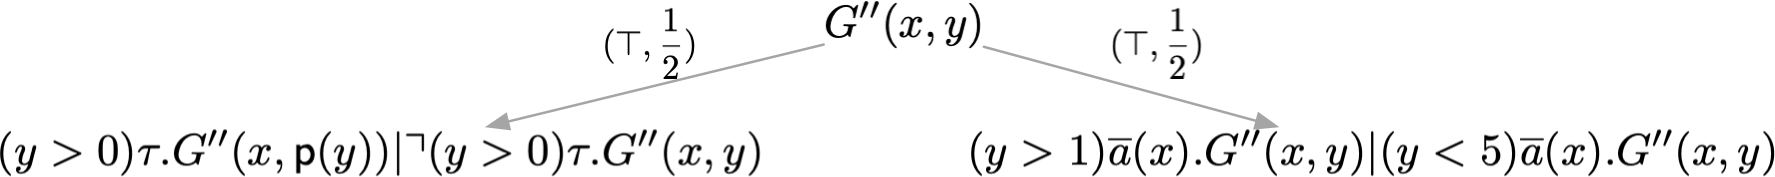
\includegraphics[width=13cm]{../figures/example4_2.png}
             \label{fig_eg4_2}
         \end{figure}

         对于$G(x)\rightsquigarrow_{\top\mathcal{S}}\stackrel{\frac{1}{2}}{\rightarrow}_{\top} [\overline{a}(x).G(x)]_{\top\mathcal{S}}$,
         存在集合$$\{G''(x,y)\rightsquigarrow_{\top\mathcal{S}}\stackrel{\frac{1}{2}}{\rightarrow}_{\top}[(y>1)\overline{a}(x).G''(x,y)|(y<5)\overline{a}(x).G''(x,y)]_{\top\mathcal{S}}\}$$
         其中$\mathsf{Th}\vdash (\top\Rightarrow\top)$且$\frac{1}{2}=\frac{1}{2}$,$(\overline{a}(x).G(x),(y>1)\overline{a}(x).G''(x,y)|(y<5)\overline{a}(x).G''(x,y))\in\mathcal{S}$。

         对于$G''(x,y)\rightsquigarrow_{\top\mathcal{S}}\stackrel{\frac{1}{2}}{\rightarrow}_{\top}[(y>1)\overline{a}(x).G''(x,y)|(y<5)\overline{a}(x).G''(x,y)]_{\top\mathcal{S}}$,
         我们可以对称地用集合$\{G(x)\rightsquigarrow_{\top\mathcal{S}}\stackrel{\frac{1}{2}}{\rightarrow}_{\top} [\overline{a}(x).G(x)]_{\top\mathcal{S}}\}$模拟。

         对于$G''(x,y)\rightsquigarrow_{\top\mathcal{S}}\stackrel{\frac{1}{2}}{\rightarrow}_{\top}[(y>0)\tau.G''(x,\mathsf{p}(y))|\urcorner(y>0)\tau.G''(x,y)]_{\top\mathcal{S}}$,
         由于等价关系具有传递性,$G''(x,y) \in [(y>0)\tau.G''(x,\mathsf{p}(y))|\urcorner(y>0)\tau.G''(x,y)]_{\top\mathcal{S}} = [G''(x,y)]_{\top\mathcal{S}}$。
      }
   \end{itemize}
   因此我们可以得出校长的判断是正确的。
\end{proof}
例~\ref{eg:5}是一个简单的例子,给出了同一系统的两种不同实现,
这两种实现在外界观察者的视角中是效果相同的,
即具有\textit{观察等价性}。
符号互模拟给观察等价性提供了严格的刻画,为观察者的\textit{主观感觉}提供了\textit{客观依据}。

\section{随机传值进程模型的等价性}

如~\ref{ch:symbolic_bisimulation}节中所述,
符号互模拟描述了$\mathbb{RVPC}_{\mathsf{Th}}$的观察等价性,
因此我们可以通过符号互模拟定义随机传值进程模型的等价性。

我们首先证明符号互模拟关系是一个等价关系,
众所周知一个等价关系应具有自反性、对称性、传递性。
根据定义~\ref{def:rvpc_symbolic_bisimulation},
容易得到符号互模拟具有自反性和对称性,
我们接下来证明符号互模拟的传递性。
\begin{lemma}\label{lemma:transitivity}
   符号互模拟具有传递性。
\end{lemma} 
\begin{proof}
   证明符号互模拟的传递性等价于证明若$\mathcal{E}$是一个符号互模拟,且$A\mathcal{E}B, B \mathcal{E} C$,则$A \mathcal{E} C$。
   \begin{itemize}
      \item {
         若$A\rightsquigarrow_{\varphi \mathcal{E}}\stackrel{\lambda}{\rightarrow}_{\varphi} \mathcal{C}\in \mathcal{T}_{RVPC}/\varphi\mathcal{E},\mathcal{C}\neq [A]_{\varphi\mathcal{E}}$,
         由于$A\mathcal{E}B$,
         根据定义存在$\varphi$的划分$\{\varphi_i\}_{i\in I}$
         和集合$S=\{B\rightsquigarrow_{\varphi_i\mathcal{E}}\stackrel{\lambda}{\rightarrow}_{\psi_i}[\mathcal{C}]_{\varphi_i\mathcal{E}}|\mathsf{Th}\vdash \varphi_i\Rightarrow\psi_i\}_{i\in I}$。
         对于$B$关于$\varphi_i\mathcal{E}$的条件等价树$t^B_{\varphi_i\mathcal{E}}$上的节点$L$,
         因为$\mathsf{Th}\vdash\varphi_i\Rightarrow \psi_i$,
         若$L\stackrel{\lambda}{\rightarrow}_{\psi_i}L'\in [\mathcal{C}]_{\varphi_i\mathcal{E}}$,
         则$L\stackrel{\lambda}{\rightarrow}_{\varphi_i}L'\in [\mathcal{C}]_{\varphi_i\mathcal{E}}$,
         因此存在集合$S'=\{B\rightsquigarrow_{\varphi_i\mathcal{E}}\stackrel{\lambda}{\rightarrow}_{\varphi_i}[\mathcal{C}]_{\varphi_i\mathcal{E}}\}_{i\in I}$,
         根据定义~\ref{def:rvpc_symbolic_bisimulation},
         $S'$也可以作为$A\rightsquigarrow_{\varphi \mathcal{E}}\stackrel{\lambda}{\rightarrow}_{\varphi} \mathcal{C}\in \mathcal{T}_{RVPC}/\varphi\mathcal{E},\mathcal{C}\neq [A]_{\varphi\mathcal{E}}$的模拟。
      
         由于$B\mathcal{E}C$,对于每一个$B\rightsquigarrow_{\varphi_i\mathcal{E}}\stackrel{\lambda}{\rightarrow}_{\varphi_i}[\mathcal{C}]_{\varphi_i\mathcal{E}}$,
         根据定义存在$\varphi_i$的划分$\{\varphi_{i,j}\}_{j\in J}$
         和集合$S_i=\{C\rightsquigarrow_{\varphi_{i,j}\mathcal{E}}\stackrel{\lambda}{\rightarrow}_{\psi_{i,j}}[\mathcal{C}]_{\varphi_{i,j}\mathcal{E}}|\mathsf{Th}\vdash \varphi_{i,j}\Rightarrow \psi_{i,j}\}_{j\in J}$,
         和集合$S_i=\{C\rightsquigarrow_{\varphi_{i,j}\mathcal{E}}\stackrel{\lambda}{\rightarrow}_{\varphi_{i,j}}[\mathcal{C}]_{\varphi_{i,j}\mathcal{E}}\}_{j\in J}$。

         进而,存在$\varphi$的划分$Con=\bigcup_{i\in I}\{\varphi_{i,j}\}_{j\in J}$
         和集合$S'=\bigcup_{i\in I}S_i'$,使得$C$可以符号模拟$A$。
         对称的证明是完全一致的。
      }
      \item {
         若$A\rightsquigarrow_{\varphi \mathcal{E}}\stackrel{q}{\rightarrow}_{\varphi} \mathcal{C}\in \mathcal{T}_{RVPC}/\varphi\mathcal{E},\mathcal{C}\neq [A]_{\varphi\mathcal{E}},q\in(0,1]$,
         由于$A\mathcal{E}B$,存在$\varphi$的划分$\{\varphi_i\}_{i\in I}$和集合$\{B\rightsquigarrow_{\varphi_i\mathcal{E}}\stackrel{q_i}{\rightarrow}_{\psi_i} [\mathcal{C}]_{\varphi_i\mathcal{E}}|\mathsf{Th}\vdash \varphi_i\Rightarrow \psi_i\wedge q=q_i\}$,
         因此存在$\{B\rightsquigarrow_{\varphi_i\mathcal{E}}\stackrel{q_i}{\rightarrow}_{\varphi_i} [\mathcal{C}]_{\varphi_i\mathcal{E}}\}$可以模拟$A$的条件$q$-迁移,
         余下部分与$l$-迁移的证明相同。
      }
   \end{itemize}
\end{proof}
证明了符号互模拟的传递性后我们可以得到定理~\ref{th:equality}。
\begin{theorem}\label{th:equality}
   符号互模拟关系是等价关系。
\end{theorem}

接下来我们希望通过符号互模拟定义$\mathbb{RVPC}_{\mathsf{Th}}$的观察等价性,
一种比较直接的想法是将$\mathbb{RVPC}_{\mathsf{Th}}$的符号互模拟的全集定义为
$\mathbb{RVPC}_{\mathsf{Th}}$的观察等价性,我们首先需要证明符号互模拟关系的全集仍然是符号互模拟关系。

\begin{lemma}\label{lemma:closure}
   如果每一个$\mathcal{T}_{\mathbb{RVPC}_{\mathsf{Th}}}$上的关系$\mathcal{E}_i$都是符号互模拟关系,
   那么$(\bigcup_{i\in I}\mathcal{E}_i)^*$是符号互模拟关系。
\end{lemma}
\begin{proof}
   令$\mathcal{E}=(\bigcup_{i\in I}\mathcal{E}_i)^*$。
   给定$A_0\mathcal{E}_{i_1}A_1\mathcal{E}_{i_2}A_2\dots A_{k-1}\mathcal{E}_{i_k} A_k$,
   由于$\mathcal{E}=(\bigcup_{i\in I}\mathcal{E}_{i})^*$,
   我们可以得到$A_1\mathcal{E}A_k$,
   若$\mathcal{E}$是一个符号互模拟关系,
   则对于条件$l$-迁移:$A_0\rightsquigarrow_{\varphi\mathcal{E}}\stackrel{\lambda}{\rightarrow}_{\varphi} \mathcal{C}\in \mathcal{T}_{\mathbb{RVPC}_{\mathsf{Th}}},\mathcal{C}\neq [A_0]_{\varphi\mathcal{E}}$,
   存在$\varphi$的划分$\{\varphi_i\}_{i\in I}$和集合
   $\{A_k\rightsquigarrow_{\varphi_i\mathcal{E}}\stackrel{\lambda}{\rightarrow}_{\psi_i}[\mathcal{C}]_{\varphi_i\mathcal{E}}|\mathsf{Th}\vdash \varphi_i\Rightarrow\psi_i\}$可模拟该操作。
   我们可以通过归纳的证明$A_0\mathcal{E}A_1$,$A_1$可以模拟$A_0$;
   $A_1\mathcal{E}A_2$,$A_2$可以模拟$A_1$;\dots;最终证明$A_k$可以模拟$A_0$。

   对于$A_0\rightsquigarrow_{\varphi\mathcal{E}}\stackrel{\lambda}{\rightarrow}_{\varphi} \mathcal{C}\in \mathcal{T}_{\mathbb{RVPC}_{\mathsf{Th}}},\mathcal{C}\neq [A_0]_{\varphi\mathcal{E}}$,
   我们需要给出$\varphi$的划分$\{\varphi_i\}_{i\in I}$
   和集合$\{A_1\rightsquigarrow_{\varphi_i\mathcal{E}}\stackrel{\lambda}{\rightarrow}_{\psi_i}[\mathcal{C}]_{\varphi_i\mathcal{E}}\}$
   来模拟$A_0$的动作。

   考虑$A_0\rightsquigarrow_{\varphi\mathcal{E}}\stackrel{\lambda}{\rightarrow}_{\varphi} \mathcal{C}\in \mathcal{T}_{\mathbb{RVPC}_{\mathsf{Th}}},\mathcal{C}\neq [A_0]_{\varphi\mathcal{E}}$,
   由等价集的定义,我们可以得出$\varphi\mathcal{E}$上的等价集$\mathcal{C}$可以被划分成不相交的$\varphi\mathcal{E}_{i_1}$上的等价集
   $\{\mathcal{C}_j^{i_1}\}$。
   假设$t_{A_0}$是$A_0$关于$\varphi\mathcal{E}$的条件等价树,
   我们可以递归的构建出$A_1$关于$\varphi\mathcal{E}$的条件等价森林。

   \begin{itemize}
      \item {
         \textbf{$t_{A_0}$的根节点$A_0$只有一个儿子节点$A_0'$。}
         若$A_0'\in[A_0]_{\varphi\mathcal{E}_{i_1}}$,
         我们将以$\varphi A_0'$作为下次递归的根节点,
         构建$\varphi A_1$条件等价森林
         (这样递归是因为在$A_1$的$\varphi\mathcal{E}$条件等价森林中的所有节点的动作都满足条件$\varphi$,
         $A_1$和$\varphi A_1$是等价的)。
         若$A_0'\notin[A_0]_{\varphi\mathcal{E}_{i_1}}$,
         根据$A_0\mathcal{E}_{i_1}A_1$,
         我们可以得到$\varphi$的划分$\{\varphi_i\}_{i\in I}$
         和集合$\{A_1\rightsquigarrow_{\varphi_i\mathcal{E}_{i_1}}\stackrel{\tau}{\rightarrow}_{\psi_i}[\mathcal{C}]_{\varphi_i\mathcal{E}_{i_1}}|\mathsf{Th}\vdash \varphi_i\Rightarrow \psi_i\}_{i\in I}$。
         
         根据推论~\ref{lemma:transitivity}的证明经验,我们其实可以用$\{A_1\rightsquigarrow_{\varphi_i\mathcal{E}_{i_1}}\stackrel{\tau}{\rightarrow}_{\varphi_i}[\mathcal{C}]_{\varphi_i\mathcal{E}_{i_1}}\}_{i\in I}$
         模拟$A_0\rightsquigarrow_{\varphi\mathcal{E}}\stackrel{\tau}{\rightarrow}_{\varphi} \mathcal{C}\in \mathcal{T}_{\mathbb{RVPC}_{\mathsf{Th}}},\mathcal{C}\neq [A_0]_{\varphi\mathcal{E}}\}_{i\in I}$,
         为了方便证明,后续的证明中我们将直接使用$\{A_1\rightsquigarrow_{\varphi_i\mathcal{E}_{i_1}}\stackrel{\lambda}{\rightarrow}_{\varphi_i}[\mathcal{C}]_{\varphi_i\mathcal{E}_{i_1}}\}_{i\in I}$的形式。
         
         $\{A_1\rightsquigarrow_{\varphi_i\mathcal{E}_{i_1}}\stackrel{\tau}{\rightarrow}_{\varphi_i}[\mathcal{C}]_{\varphi_i\mathcal{E}_{i_1}}\}_{i\in I}$
         实际构建出了一个条件等价树的集合$\{t_{A_1}^{i}\}_{i\in I}$,
         对于每个条件等价树$t_{A_1}^i$的叶子节点$B$,$B\stackrel{\tau}{\rightarrow}_{\varphi_i}B'\in [A_0']_{\varphi_i\mathcal{E}_{i_1}}$,
         我们根据$\varphi_i A_0'$构建每一个$\varphi_i B'$关于$\varphi_i\mathcal{E}$的等价森林。
         此时将$B$所在的$\varphi_i\mathcal{E}$等价树$t_{A_1}^{i}$复制并
         与每个$B'$的$\varphi_i\mathcal{E}$的等价森林中的等价树相连,
         我们可以得到$A_1$关于$\varphi\mathcal{E}$的条件等价森林。
      }
      \item {
         \textbf{$t_{A_0}$的根节点$A_0$有$h$个儿子节点$A_0^1,\dots,A_0^h$。}
         根据定义$A_0\stackrel{\coprod_{i\in [h]p_j\tau}}{\rightarrow}_{\psi} \coprod_{j\in [h]}A_0^j$,
         $A_0$到$A_0^j$的边被标记为$(\psi, p_j)$,其中$\varphi\Rightarrow\psi$。

         若所有$A_0^j\in [A_0]_{\varphi\mathcal{E}_{i_1}}$,
         我们将根据$\varphi A_0^1$构建$\varphi A_1$的条件等价森林。

         若存在$A_0^j\notin [A_0]_{\varphi\mathcal{E}_{i_1}}$,
         不妨设为$A_0^1$,则$A_0\rightsquigarrow_{\varphi\mathcal{E}_{i_1}}\stackrel{q}{\rightarrow}_{\varphi} [A_0^1]_{\varphi\mathcal{E}_{i_1}}$,
         根据$A_0\mathcal{E}_{i_1}A_1$,
         我们可以得到$\varphi$的划分$\{\varphi_i\}_{i\in I}$和集合
         $\{A_1\rightsquigarrow_{\varphi_i\mathcal{E}_{i_1}}\stackrel{q}{\rightarrow}_{\varphi_i} [A_0^1]_{\varphi_i\mathcal{E}_{i_1}}\}_{i\in I}$,
         这其中关系到$A_1$关于$\varphi_i\mathcal{E}_{i_1}$的条件等价树$t_1^i$,
         根据条件$q$-迁移的定义,
         存在$\mathsf{P}_{\varphi_i,\varphi_i\mathcal{E}_{i_1}}(N\stackrel{\coprod_{i'\in [h']}p_{i'}\tau}{\longrightarrow}_{\varphi_i} N'\in [A_0^1]_{\varphi_i\mathcal{E}_{i_1}}) = q$,
         我们根据$\varphi_i A_0^1$构建每个$\varphi_i N'$关于$\varphi_i\mathcal{E}$的条件等价森林。
      }
      \item {
         \textbf{$t_{A_0}$的根节点$A_0$可以作$A_0\stackrel{\lambda}{\rightarrow}_{\varphi} L'$。}
         根据定义存在$\varphi$的划分$\{\varphi_i\}_{i\in I}$和集合
         $\{A_1\rightsquigarrow_{\varphi_i\mathcal{E}_{i_1}}\stackrel{\lambda}{\rightarrow}_{\varphi_i} [L']_{\varphi_i\mathcal{E}_{i_1}}\}$。
      }
   \end{itemize}

   上述递归的构建可以通过图~\ref{fig:equal_forest}更加形象的表述。
   \begin{figure}[!htbp]
      \small
      \centering
      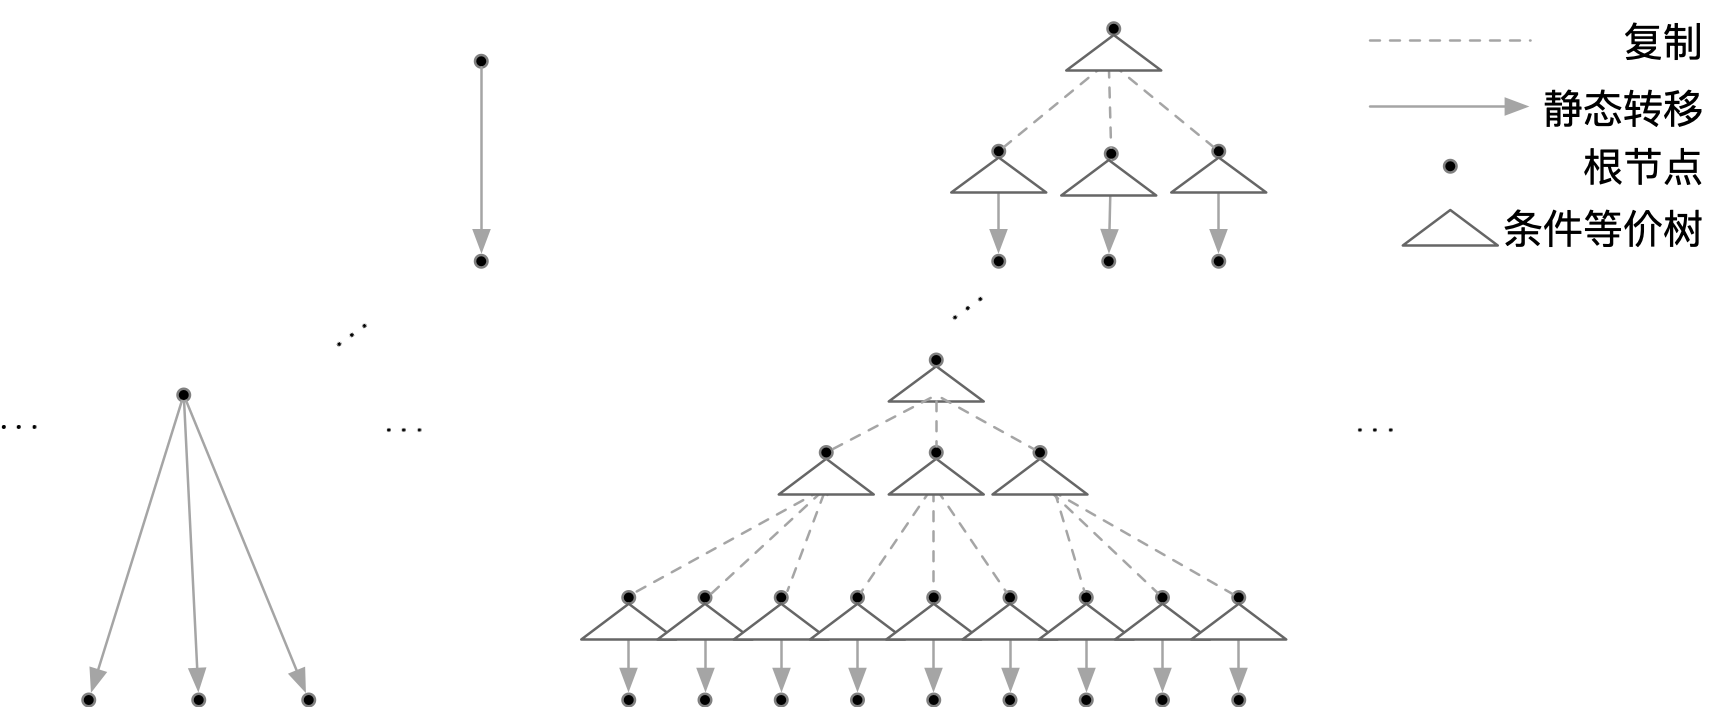
\includegraphics[width=13cm]{../figures/equality_1.png}
      \caption[]{递归构建图解} 
      \label{fig:equal_forest}
   \end{figure}
   图~\ref{fig:equal_forest}中,
   第一层描述了根节点只有一个儿子节点情况的构建方法,
   对于每一个$i\in I$,
   右侧的条件等价树都会复制一份,
   全部的条件等价树构成$\varphi\mathcal{E}$条件等价森林,
   作$\{A_1\rightsquigarrow_{\varphi_i\mathcal{E}_{i_1}\stackrel{\tau}{\rightarrow}_{\varphi_i}}[A_0']_{\varphi_i\mathcal{E}_{i_1}}\}$
   对$A_0\stackrel{\tau}{\rightarrow}_{\varphi\mathcal{E}_{i_1}}A_0'$的模拟。

   第二层描述了根节点有多个儿子节点情况的构建方法,
   对于每一个$A_0\rightsquigarrow_{\varphi\mathcal{E}_{i_1}}\stackrel{q}{\rightarrow}_{\varphi}$,
   右侧的条件等价树会复制一份,
   在对每一个$A_0\rightsquigarrow_{\varphi\mathcal{E}_{i_1}}\stackrel{q}{\rightarrow}_{\varphi} [A_0^1]_{\varphi\mathcal{E}_{i_1}}$
   模拟时,对模拟该动作的集合$\{A_1\rightsquigarrow_{\varphi_i\mathcal{E}_{i_1}}\stackrel{q}{\rightarrow}_{\varphi_i} [A_0^1]_{\varphi_i\mathcal{E}_{i_1}}\}_{i\in I}$
   中的每一个元素都复制一份条件等价树,再进行对应的模拟。

   通过上述构建方式,我们最终会构建出$A_1$关于$\varphi\mathcal{E}$的条件等价树或条件等价森林,
   来模拟$A_0\rightsquigarrow_{\varphi\mathcal{E}}\stackrel{\lambda}{\rightarrow}_{\varphi} \mathcal{C}\in \mathcal{T}_{\mathbb{RVPC}_{\mathsf{Th}}},\mathcal{C}\neq [A_0]_{\varphi\mathcal{E}}$。
   归纳地,我们可以构建出$A_2$对$A_1$关于$\varphi\mathcal{E}$的条件等价树或条件等价森林中的每一个条件等价树的迁移
   的条件等价森林……最终构建出$A_k$模拟$A_0\rightsquigarrow_{\varphi\mathcal{E}}\stackrel{\lambda}{\rightarrow}_{\varphi} \mathcal{C}\in \mathcal{T}_{\mathbb{RVPC}_{\mathsf{Th}}},\mathcal{C}\neq [A_0]_{\varphi\mathcal{E}}$的条件等价森林。

   对于条件$q$-迁移:$A_0\rightsquigarrow_{\varphi\mathcal{E}}\stackrel{q}{\rightarrow}_{\varphi}\mathcal{C}$的证明方法是相同的。
\end{proof}

我们希望定义符号互模拟关系的全集为$\mathbb{RVPC}_{\mathsf{Th}}$上的观察等价性,
但这样定义仍会存在问题:考虑$A\in\mathcal{T}_{\mathbb{RVPC}_{\mathsf{Th}}}$,
若$A$在$\varphi\mathcal{E}$下的条件等价树是无限延伸的,即没有叶子节点,
这时找到$A$的条件$l$转移和条件$q$转移就会变得困难,因此我们引入Uniform Approach中的codivergent的相关概念来解决这个问题。

\begin{definition}\label{def:divergent}
   对于$A\in\mathcal{T}_{\mathbb{RVPC}_{\mathsf{Th}}}$,
   若$A$在$\varphi\mathcal{E}$下的条件等价树为$t$,
   定义树$t$的分支$\pi$是$t$从根节点开始到叶节点结束的一条路径,
   定义$\pi(i)$为分支$\pi$上第$i$条边的标记中的概率部分,$\pi(i)\in(0,1]$。

   定义这条分支的概率$\mathsf{P}(\pi)=\prod\{\pi(i)|i\in [|\pi|]\}$,
   若这条分支是无穷的,则$\mathsf{P}(\pi)=\lim_{j\rightarrow \infty}\prod_{i=0}^{i=j}\pi(i)$。

   定义条件等价树的概率$\mathsf{P}(t)=\sum\{\mathsf{P}(\pi)|\pi\textrm{是}t\textrm{的一条分支}\}$。
   
   定义$t$的前$k$层分支的概率为$\mathsf{P}^k(t)=\sum \{\mathsf{P}(\pi)|\pi\textrm{是}t\textrm{的一条分支且}|\pi|\leq k\}$。

   定义$t$的有限长分支的概率$\mathsf{P}^f(t)=\lim_{k\rightarrow\infty}\mathsf{P}^k(t)$。

   当条件等价树$t$的有限长分支的概率$\mathsf{P}^f(t)=0$时,
   $t$称为\textit{发散的条件等价树},我们可以理解为$t$没有有限长的分支。
\end{definition}

通过定义~\ref{def:divergent},我们定义了使用符号互模拟关系的全集作为观察等价性时,
存在问题的情况,我们使用共发散(codivergent)的概念对这种情况的条件等价树的观察等价性单独定义。

\begin{definition}
   若$\mathcal{E}$是$\mathcal{T}_{\mathbb{RVPC}_{\mathsf{Th}}}$上的等价关系,
   $\mathcal{E}$是一个共发散的等价关系当且仅当:
   当对于所有的布尔表达式$\varphi$,
   对条件等价集$\mathcal{C}\in\mathcal{T}_{\mathbb{RVPC}_{\mathsf{Th}}}/\varphi\mathcal{E}$,
   $\mathcal{C}$中的每一个元素关于$\varphi\mathcal{E}$的条件等价森林中的每一个棵树都是发散的等价树;
   或$\mathcal{C}$中的每一个元素关于$\varphi\mathcal{E}$的条件等价森林中的每一个棵树都不是是发散的等价树。
\end{definition}

\begin{definition}
   $\mathcal{T}_{\mathbb{RVPC}_{\mathsf{Th}}}$上的观察等价性$=_{\mathbb{RVPC}_{\mathsf{Th}}}$定义为$\mathcal{T}_{\mathbb{RVPC}_{\mathsf{Th}}}$上的共发散的符号互模拟关系的全集。
\end{definition}
由于$=_{\mathbb{RVPC}_{\mathsf{Th}}}$仍然是一个符号互模拟关系,因此我们可以得到定理~\ref{th:equality2}。
\begin{theorem}\label{th:equality2}
   $=_{\mathbb{RVPC}_{\mathsf{Th}}}$是一个等价关系。
\end{theorem}

在数学特别是抽象代数中,同余关系或简称同余是相容于某个代数运算的等价关系。
设$A=<S,*,\delta>$是一个代数系统,$\sim$是载体$S$上的等价关系,若$\sim$在$A$上的所有运算下都是可保持的,则称$\sim$为代数系统$A$上的同余关系\cite{Cougruence}。 
同余关系使得元素所在的等价类在运算上可以作为一个整体来看待。
我们希望证明我们定义的$=_{\mathbb{RVPC}_{\mathsf{Th}}}$是一个同余关系。

\begin{theorem}
   $=_{\mathbb{RVPC}_{\mathsf{Th}}}$具有同余性。
\end{theorem}
\begin{proof}
   $=_{\mathbb{RVPC}_{\mathsf{Th}}}$对于随机选择和非确定性选择的可保持性比较容易证明。
   由推论~\ref{co:condition}易知$A=_{\mathbb{RVPC}_{\mathsf{Th}}}B$则$\varphi A=_{\mathbb{RVPC}_{\mathsf{Th}}}\varphi B$。
   为方便证明,以下$=_{\mathbb{RVPC}_{\mathsf{Th}}}$简记为$=$,绝对等价性记为$\equiv$,定义记为$\stackrel{def}{=}$。
   
   对于本地化操作子(Localization),对于$A=B,(a)A\rightsquigarrow_{\varphi=}\stackrel{\lambda}{\rightarrow}_{\varphi} (a)A'\notin [(a)A]_{\varphi =}, a\notin \lambda$,
   易知有$\varphi$的划分$\{\varphi_i\}_{i\in I}$和集合$\{(a)B\rightsquigarrow_{\varphi_i=}\stackrel{\lambda}{\rightarrow}_{\varphi_i}[(a)A]_{\varphi =}\}$。

   对于并发操作子(Composition),考虑等价关系$\mathcal{R}\stackrel{def}{=}\{(A|C,B|D)|(A,B)\in =,(C,D)\in =\}$,
   令$\mathcal{R}' = (\mathcal{R}\cup =)^*$,我们证明$\mathcal{R}'$是一个符号互模拟关系。
   对于条件$l$-迁移:$(A|C)\rightsquigarrow_{\varphi\mathcal{R'}}\stackrel{\lambda}{\rightarrow}_{\varphi}\mathcal{C}\in\mathcal{T}_{\mathbb{RVPC}_{\mathsf{Th}}}/\varphi \mathcal{R}',\mathcal{C}\neq [(A|C)]_{\varphi\mathcal{R}'}$,
   我们可以用引理~\ref{lemma:closure}中的方法递归的构造$(B|C)$的$\varphi\mathcal{E}$条件等价森林来模拟$(A|C)$的动作,
   令$t_{(A|C)}$为$(A|C)$关于$\varphi\mathcal{R'}$的条件等价树。
   \begin{itemize}
      \item {
         $t_{(A|C)}$上的边:
         $A|C\stackrel{(\psi, 1)}{\rightarrow} A'|C, \mathsf{Th}\vdash \varphi\Rightarrow\psi$
         是由于$A\stackrel{\tau}{\rightarrow}_{\varphi} A'$。

         若$A'\in [A]_{\varphi =}$,
         那么$(A'|C)\in[(A|C)]_{\varphi\mathcal{R}'}\equiv[(B|D)]_{\varphi\mathcal{R}'}$。
         实际上,对于$A\stackrel{\coprod_{i\in I}p_i\tau}{\rightarrow}_{\varphi} \coprod_{i\in I} A_i=A$,
         $A_i|C\in [B|D]_{\varphi\mathcal{R}'}$。
         我们可以根据$\varphi (A_0|C)$的$\varphi\mathcal{R}'$条件等价树构建$(B|D)$的$\varphi\mathcal{R}'$条件等价森林。

         若$A'\notin [A]_{\varphi =}$,
         那么根据定义存在$\{B\rightsquigarrow_{\varphi_i\mathcal{=}}\stackrel{\tau}{\rightarrow}_{\varphi_i}B_i\in [A']_{\varphi_i =}\}_{i\in I}$,
         模拟$A\rightsquigarrow_{\varphi =}\stackrel{\tau}{\rightarrow}_{\varphi} A'$,
         其中$\{\varphi_i\}_{i\in I}$是$\varphi$的划分。
         我们根据$\varphi_i A'$构建$\varphi_i B_i$的$\varphi_i \mathcal{R}'$条件等价森林。
      }
      \item {
         $t_{(A|C)}$上的边:
         $A|C\stackrel{(\psi, 1)}{\rightarrow} A'|C', \mathsf{Th}\vdash \varphi\Rightarrow\psi$
         是由于$A\stackrel{\overline{a}(t)}{\longrightarrow}_{\psi'} A', C\stackrel{a(x)}{\longrightarrow}_{\psi''} C', \psi=\psi'\psi''$。

         根据$A=B,C=D$,
         $A\rightsquigarrow_{\varphi = }\stackrel{\overline{a}(t)}{\longrightarrow}_{\varphi}A'$
         可以由$\{B\rightsquigarrow_{\varphi_i =}\stackrel{\overline{a}(t)}{\longrightarrow}_{\varphi_i}B_i\in [A']_{\varphi_i=}\}_{i\in I}$模拟,
         其中$\{\varphi_i\}_{i\in I}$是$\varphi$的划分。
         $C\rightsquigarrow_{\varphi = }\stackrel{a(x)}{\longrightarrow}_{\varphi}C'$
         可以由$\{D\rightsquigarrow_{\varphi_j =}\stackrel{a(x)}{\longrightarrow}_{\varphi_j}D_j\in [C']_{\varphi_j=}\}_{j\in J}$模拟,
         其中$\{\varphi_j\}_{j\in J}$是$\varphi$的划分。

         对于所有的$i\in I, j\in J, \mathsf{Th}\vdash \varphi_i\varphi_j\not\Rightarrow \bot$,
         $(B_i\mid D_j)\in[A'\mid C']_{\varphi_i\varphi_j \mathcal{R'}}$,
         我们根据$\varphi_i\varphi_j(A'|C')$的$\varphi_i\varphi_j \mathcal{R}' $条件等价树构建$\varphi_i\varphi_j(B_i|D_j)$的$\varphi_i\varphi_j \mathcal{R}' $条件等价森林。
      }
      \item {
         $t_{(A|C)}$上的边:
         $A|C\stackrel{(\psi, q)}{\rightarrow} A'|C, \mathsf{Th}\vdash \varphi\Rightarrow\psi, q\in(0,1)$,
         则存在$A\stackrel{\coprod_{i\in I}p_i\tau}{\longrightarrow}_{\varphi} \coprod_{i\in I} A_i$,
         对所有的$i\in I$,$A|C\stackrel{(\psi, p_i)}{\rightarrow} A_i|C, \mathsf{Th}\vdash \varphi\Rightarrow\psi$。

         若对所有的$i\in I, A_i\in[A]_{\varphi =}$,我们可以根据$(A_i|C)$关于$\varphi\mathcal{R}'$的条件等价树构建$(B|D)$的$\varphi\mathcal{R}'$条件等价森林。

         若存在$A_i\notin [A]_{\varphi =}$,不妨设为$A_0$,
         若有$A_1\notin[A]_{\varphi =}\wedge A_1\in [A_0]_{\varphi =}$,
         此时有$A\rightsquigarrow_{\varphi = }\stackrel{q_0}{\rightarrow}_{\varphi}[A_0]_{\varphi=}$,
         $A\rightsquigarrow_{\varphi = }\stackrel{q_1}{\rightarrow}_{\varphi}[A_0]_{\varphi=}$,
         $A|C\rightsquigarrow_{\varphi = }\stackrel{q_0+q_1}{\longrightarrow}_{\varphi}[A_1|C]_{\varphi=}$。

         根据$A=B$,存在$\varphi$的划分$\{\varphi_i\}_{i\in I}$和集合
         $\{B\rightsquigarrow_{\varphi_i=}\stackrel{q_0}{\rightarrow}_{\varphi_i}B_i\in [A_0]_{\varphi_i =}\}$
         模拟$A\rightsquigarrow_{\varphi = }\stackrel{q_0}{\rightarrow}_{\varphi}[A_0]_{\varphi=}$。
         存在$\varphi$的划分$\{\varphi_j\}_{j\in J}$和集合
         $\{B\rightsquigarrow_{\varphi_j=}\stackrel{q_1}{\rightarrow}_{\varphi_j}B_j\in [A_1]_{\varphi_j =}\}$
         模拟$A\rightsquigarrow_{\varphi = }\stackrel{q_1}{\rightarrow}_{\varphi}[A_1]_{\varphi=}$。
         对所有的$i\in I, j\in J, \mathsf{Th}\vdash \varphi_i\varphi_j\not\Rightarrow \bot$,
         我们有$(B|D)\rightsquigarrow_{\varphi_i\varphi_j=}\stackrel{q_0+q_1}{\longrightarrow}_{\varphi_i\varphi_j}(B'|D)\in[A_0|C]_{\varphi_i\varphi_j=}$,
         我们根据$\varphi_i\varphi_j (A_0|C)$的$\varphi_i\varphi_j \mathcal{R}' $条件等价树构建$\varphi_i\varphi_j(B'|D)$的$\varphi_i\varphi_j \mathcal{R}' $条件等价森林。
      }
      \item {
         若$(A|C)\stackrel{\lambda}{\rightarrow}_{\varphi} (A'|C), \lambda\neq \tau$,
         则$A\stackrel{\lambda}{\rightarrow}_{\varphi} A'$,
         根据定义存在$\varphi$的划分$\{\varphi_i\}_{i\in I}$和集合
         $\{B|D\rightsquigarrow_{\varphi_i=}\stackrel{\lambda}{\rightarrow}_{\varphi_i} [(A'|C)]_{\varphi_i=}\}$。
      }
   \end{itemize}
   对于条件$q$-迁移:$(A|C)\rightsquigarrow_{\varphi=}\stackrel{q}{\rightarrow}_{\varphi}\mathcal{C}$的证明方法是相同的。

   在上述证明中,若$(A,B)\in =$,且$A$关于$\varphi =$的条件等价树是发散的,
   根据定义可知$B$对应的条件等价森林中的条件等价树也是发散的,
   我们可以根据同样的扩展方法证明共发散对上述操作子的同余性。
\end{proof}

\section{本章小结}
本章我们介绍了一种经典的并发进程模型——传值进程模型(The Value-Passing Calculus)和它的一种实现$\mathbb{VPC}_{\mathsf{Th}}$,
并使用Uniform Approach中的方法为$\mathbb{VPC}_{\mathsf{Th}}$添加了随机选择操作子,
扩展成为随机传值进程模型$\mathbb{RVPC}_{\mathsf{Th}}$,
给出了随机传值进程模型$\mathbb{RVPC}_{\mathsf{Th}}$的语法和迁移语义。

为了给出$\mathbb{RVPC}_{\mathsf{Th}}$观察等价性的定义,
我们引入了$\mathbb{VPC}_{\mathbb{Th}}$中的等价集、符号互模拟的概念,
由于$\mathbb{RVPC}_{\mathsf{Th}}$中涉及到条件操作子,
我们将等价集的概念扩展为条件等价集,
在此基础上使用Uniform Approach的方法给出了
$\mathcal{T}_{\mathbb{RVPC}_{\mathsf{Th}}}$的条件等价树的概念,
并使用条件等价树给出了$\mathcal{T}_{\mathbb{RVPC}_{\mathsf{Th}}}$的符号互模拟关系的定义。
为了解决无限的条件等价树无法得到符号互模拟关系的问题,
我们根据Uniform Approach提出了$\mathbb{RVPC}_{\mathsf{Th}}$上共发散的定义,
我们将共发散的符号互模拟的全集定义为$\mathbb{RVPC}_{\mathsf{Th}}$的观察等价性,
并证明了$\mathbb{RVPC}_{\mathsf{Th}}$观察等价性是一个同余关系。